\documentclass[]{article}
\usepackage{lmodern}
\usepackage{amssymb,amsmath}
\usepackage{ifxetex,ifluatex}
\usepackage{fixltx2e} % provides \textsubscript
\ifnum 0\ifxetex 1\fi\ifluatex 1\fi=0 % if pdftex
  \usepackage[T1]{fontenc}
  \usepackage[utf8]{inputenc}
\else % if luatex or xelatex
  \ifxetex
    \usepackage{mathspec}
  \else
    \usepackage{fontspec}
  \fi
  \defaultfontfeatures{Ligatures=TeX,Scale=MatchLowercase}
\fi
% use upquote if available, for straight quotes in verbatim environments
\IfFileExists{upquote.sty}{\usepackage{upquote}}{}
% use microtype if available
\IfFileExists{microtype.sty}{%
\usepackage{microtype}
\UseMicrotypeSet[protrusion]{basicmath} % disable protrusion for tt fonts
}{}
\usepackage[margin=1in]{geometry}
\usepackage{hyperref}
\hypersetup{unicode=true,
            pdfborder={0 0 0},
            breaklinks=true}
\urlstyle{same}  % don't use monospace font for urls
\usepackage{color}
\usepackage{fancyvrb}
\newcommand{\VerbBar}{|}
\newcommand{\VERB}{\Verb[commandchars=\\\{\}]}
\DefineVerbatimEnvironment{Highlighting}{Verbatim}{commandchars=\\\{\}}
% Add ',fontsize=\small' for more characters per line
\usepackage{framed}
\definecolor{shadecolor}{RGB}{248,248,248}
\newenvironment{Shaded}{\begin{snugshade}}{\end{snugshade}}
\newcommand{\KeywordTok}[1]{\textcolor[rgb]{0.13,0.29,0.53}{\textbf{#1}}}
\newcommand{\DataTypeTok}[1]{\textcolor[rgb]{0.13,0.29,0.53}{#1}}
\newcommand{\DecValTok}[1]{\textcolor[rgb]{0.00,0.00,0.81}{#1}}
\newcommand{\BaseNTok}[1]{\textcolor[rgb]{0.00,0.00,0.81}{#1}}
\newcommand{\FloatTok}[1]{\textcolor[rgb]{0.00,0.00,0.81}{#1}}
\newcommand{\ConstantTok}[1]{\textcolor[rgb]{0.00,0.00,0.00}{#1}}
\newcommand{\CharTok}[1]{\textcolor[rgb]{0.31,0.60,0.02}{#1}}
\newcommand{\SpecialCharTok}[1]{\textcolor[rgb]{0.00,0.00,0.00}{#1}}
\newcommand{\StringTok}[1]{\textcolor[rgb]{0.31,0.60,0.02}{#1}}
\newcommand{\VerbatimStringTok}[1]{\textcolor[rgb]{0.31,0.60,0.02}{#1}}
\newcommand{\SpecialStringTok}[1]{\textcolor[rgb]{0.31,0.60,0.02}{#1}}
\newcommand{\ImportTok}[1]{#1}
\newcommand{\CommentTok}[1]{\textcolor[rgb]{0.56,0.35,0.01}{\textit{#1}}}
\newcommand{\DocumentationTok}[1]{\textcolor[rgb]{0.56,0.35,0.01}{\textbf{\textit{#1}}}}
\newcommand{\AnnotationTok}[1]{\textcolor[rgb]{0.56,0.35,0.01}{\textbf{\textit{#1}}}}
\newcommand{\CommentVarTok}[1]{\textcolor[rgb]{0.56,0.35,0.01}{\textbf{\textit{#1}}}}
\newcommand{\OtherTok}[1]{\textcolor[rgb]{0.56,0.35,0.01}{#1}}
\newcommand{\FunctionTok}[1]{\textcolor[rgb]{0.00,0.00,0.00}{#1}}
\newcommand{\VariableTok}[1]{\textcolor[rgb]{0.00,0.00,0.00}{#1}}
\newcommand{\ControlFlowTok}[1]{\textcolor[rgb]{0.13,0.29,0.53}{\textbf{#1}}}
\newcommand{\OperatorTok}[1]{\textcolor[rgb]{0.81,0.36,0.00}{\textbf{#1}}}
\newcommand{\BuiltInTok}[1]{#1}
\newcommand{\ExtensionTok}[1]{#1}
\newcommand{\PreprocessorTok}[1]{\textcolor[rgb]{0.56,0.35,0.01}{\textit{#1}}}
\newcommand{\AttributeTok}[1]{\textcolor[rgb]{0.77,0.63,0.00}{#1}}
\newcommand{\RegionMarkerTok}[1]{#1}
\newcommand{\InformationTok}[1]{\textcolor[rgb]{0.56,0.35,0.01}{\textbf{\textit{#1}}}}
\newcommand{\WarningTok}[1]{\textcolor[rgb]{0.56,0.35,0.01}{\textbf{\textit{#1}}}}
\newcommand{\AlertTok}[1]{\textcolor[rgb]{0.94,0.16,0.16}{#1}}
\newcommand{\ErrorTok}[1]{\textcolor[rgb]{0.64,0.00,0.00}{\textbf{#1}}}
\newcommand{\NormalTok}[1]{#1}
\usepackage{graphicx,grffile}
\makeatletter
\def\maxwidth{\ifdim\Gin@nat@width>\linewidth\linewidth\else\Gin@nat@width\fi}
\def\maxheight{\ifdim\Gin@nat@height>\textheight\textheight\else\Gin@nat@height\fi}
\makeatother
% Scale images if necessary, so that they will not overflow the page
% margins by default, and it is still possible to overwrite the defaults
% using explicit options in \includegraphics[width, height, ...]{}
\setkeys{Gin}{width=\maxwidth,height=\maxheight,keepaspectratio}
\IfFileExists{parskip.sty}{%
\usepackage{parskip}
}{% else
\setlength{\parindent}{0pt}
\setlength{\parskip}{6pt plus 2pt minus 1pt}
}
\setlength{\emergencystretch}{3em}  % prevent overfull lines
\providecommand{\tightlist}{%
  \setlength{\itemsep}{0pt}\setlength{\parskip}{0pt}}
\setcounter{secnumdepth}{0}
% Redefines (sub)paragraphs to behave more like sections
\ifx\paragraph\undefined\else
\let\oldparagraph\paragraph
\renewcommand{\paragraph}[1]{\oldparagraph{#1}\mbox{}}
\fi
\ifx\subparagraph\undefined\else
\let\oldsubparagraph\subparagraph
\renewcommand{\subparagraph}[1]{\oldsubparagraph{#1}\mbox{}}
\fi

%%% Use protect on footnotes to avoid problems with footnotes in titles
\let\rmarkdownfootnote\footnote%
\def\footnote{\protect\rmarkdownfootnote}

%%% Change title format to be more compact
\usepackage{titling}

% Create subtitle command for use in maketitle
\newcommand{\subtitle}[1]{
  \posttitle{
    \begin{center}\large#1\end{center}
    }
}

\setlength{\droptitle}{-2em}
  \title{}
  \pretitle{\vspace{\droptitle}}
  \posttitle{}
  \author{}
  \preauthor{}\postauthor{}
  \date{}
  \predate{}\postdate{}


\begin{document}

\section{The effect of QUD and prior on exhaustivity: an empirical
investigation}\label{the-effect-of-qud-and-prior-on-exhaustivity-an-empirical-investigation}

\subsection{Part 1: Set-up}\label{part-1-set-up}

Installing packages:

\begin{Shaded}
\begin{Highlighting}[]
\KeywordTok{library}\NormalTok{(tidyverse)}
\end{Highlighting}
\end{Shaded}

\begin{verbatim}
## -- Attaching packages ----------------------------------------------------------------------- tidyverse 1.2.1 --
\end{verbatim}

\begin{verbatim}
## √ ggplot2 2.2.1     √ purrr   0.2.4
## √ tibble  1.4.2     √ dplyr   0.7.4
## √ tidyr   0.8.0     √ stringr 1.3.0
## √ readr   1.1.1     √ forcats 0.2.0
\end{verbatim}

\begin{verbatim}
## -- Conflicts -------------------------------------------------------------------------- tidyverse_conflicts() --
## x dplyr::filter() masks stats::filter()
## x dplyr::lag()    masks stats::lag()
\end{verbatim}

\begin{Shaded}
\begin{Highlighting}[]
\KeywordTok{library}\NormalTok{(brms)}
\end{Highlighting}
\end{Shaded}

\begin{verbatim}
## Loading required package: Rcpp
\end{verbatim}

\begin{verbatim}
## Warning: package 'Rcpp' was built under R version 3.4.4
\end{verbatim}

\begin{verbatim}
## Loading 'brms' package (version 2.3.1). Useful instructions
## can be found by typing help('brms'). A more detailed introduction
## to the package is available through vignette('brms_overview').
## Run theme_set(theme_default()) to use the default bayesplot theme.
\end{verbatim}

\begin{Shaded}
\begin{Highlighting}[]
\KeywordTok{library}\NormalTok{(forcats)}
\KeywordTok{library}\NormalTok{(stringr)}
\KeywordTok{library}\NormalTok{(lme4)}
\end{Highlighting}
\end{Shaded}

\begin{verbatim}
## Warning: package 'lme4' was built under R version 3.4.4
\end{verbatim}

\begin{verbatim}
## Loading required package: Matrix
\end{verbatim}

\begin{verbatim}
## 
## Attaching package: 'Matrix'
\end{verbatim}

\begin{verbatim}
## The following object is masked from 'package:tidyr':
## 
##     expand
\end{verbatim}

\begin{verbatim}
## 
## Attaching package: 'lme4'
\end{verbatim}

\begin{verbatim}
## The following object is masked from 'package:brms':
## 
##     ngrps
\end{verbatim}

\begin{Shaded}
\begin{Highlighting}[]
\KeywordTok{library}\NormalTok{(languageR)}
\KeywordTok{library}\NormalTok{(ggrepel)}
\end{Highlighting}
\end{Shaded}

\begin{verbatim}
## Warning: package 'ggrepel' was built under R version 3.4.4
\end{verbatim}

Setting theme for visualizations and adding Judith's helper functions
file

\begin{Shaded}
\begin{Highlighting}[]
\KeywordTok{theme_set}\NormalTok{(}\KeywordTok{theme_bw}\NormalTok{(}\DecValTok{18}\NormalTok{))}
\KeywordTok{source}\NormalTok{(}\StringTok{"helpers.r"}\NormalTok{)}
\end{Highlighting}
\end{Shaded}

Reading in the data from the critical experiment and the norming
experiment where prior beliefs were collected

\begin{Shaded}
\begin{Highlighting}[]
\NormalTok{d1 =}\StringTok{ }\KeywordTok{read.table}\NormalTok{(}\DataTypeTok{file=}\StringTok{"../data/1_critical/experiment1.csv"}\NormalTok{,}\DataTypeTok{sep=}\StringTok{","}\NormalTok{, }\DataTypeTok{header=}\NormalTok{T)}
\NormalTok{d1}\OperatorTok{$}\NormalTok{workerid =}\StringTok{ }\NormalTok{d1}\OperatorTok{$}\NormalTok{workerid }\OperatorTok{+}\StringTok{ }\DecValTok{300}
\NormalTok{d2 =}\StringTok{ }\KeywordTok{read.table}\NormalTok{(}\DataTypeTok{file=}\StringTok{"../data/1_critical/experiment2.csv"}\NormalTok{,}\DataTypeTok{sep=}\StringTok{","}\NormalTok{, }\DataTypeTok{header=}\NormalTok{T)}
\NormalTok{d =}\StringTok{ }\KeywordTok{rbind}\NormalTok{(d1,d2)}
\CommentTok{# d = read.table(file="../data/1_critical/pilot.csv",sep=",", header=T)}
\NormalTok{d =}\StringTok{ }\KeywordTok{as.data.frame}\NormalTok{(}\KeywordTok{lapply}\NormalTok{(d, }\ControlFlowTok{function}\NormalTok{(x) \{}\KeywordTok{gsub}\NormalTok{(}\StringTok{'}\CharTok{\textbackslash{}"}\StringTok{'}\NormalTok{,}\StringTok{""}\NormalTok{,x)\}))}
\NormalTok{priors =}\StringTok{ }\KeywordTok{read.table}\NormalTok{(}\DataTypeTok{file=}\StringTok{"../data/1_norm/experiment.csv"}\NormalTok{,}\DataTypeTok{sep=}\StringTok{","}\NormalTok{, }\DataTypeTok{header=}\NormalTok{T)}
\NormalTok{priors =}\StringTok{ }\KeywordTok{as.data.frame}\NormalTok{(}\KeywordTok{lapply}\NormalTok{(priors, }\ControlFlowTok{function}\NormalTok{(x) \{}\KeywordTok{gsub}\NormalTok{(}\StringTok{'}\CharTok{\textbackslash{}"}\StringTok{'}\NormalTok{,}\StringTok{""}\NormalTok{,x)\}))}
\end{Highlighting}
\end{Shaded}

Ensuring that different variables are correctly assigned as factors,
numbers, and strings

\begin{Shaded}
\begin{Highlighting}[]
\NormalTok{d}\OperatorTok{$}\NormalTok{Trial =}\StringTok{ }\KeywordTok{as.numeric}\NormalTok{(}\KeywordTok{as.character}\NormalTok{(d}\OperatorTok{$}\NormalTok{slide_number)) }\OperatorTok{-}\StringTok{ }\DecValTok{3}
\NormalTok{d}\OperatorTok{$}\NormalTok{Answer.time_in_minutes =}\StringTok{ }\KeywordTok{as.numeric}\NormalTok{(}\KeywordTok{as.character}\NormalTok{(d}\OperatorTok{$}\NormalTok{Answer.time_in_minutes))}
\NormalTok{d}\OperatorTok{$}\NormalTok{age =}\StringTok{ }\KeywordTok{as.numeric}\NormalTok{(}\KeywordTok{as.character}\NormalTok{(d}\OperatorTok{$}\NormalTok{age))}
\NormalTok{d}\OperatorTok{$}\NormalTok{topic =}\StringTok{ }\KeywordTok{as.factor}\NormalTok{(}\KeywordTok{as.character}\NormalTok{(d}\OperatorTok{$}\NormalTok{topic))}
\NormalTok{d}\OperatorTok{$}\NormalTok{slide_number =}\StringTok{ }\KeywordTok{as.numeric}\NormalTok{(}\KeywordTok{as.character}\NormalTok{(d}\OperatorTok{$}\NormalTok{slide_number))}

\NormalTok{priors}\OperatorTok{$}\NormalTok{response =}\StringTok{ }\KeywordTok{as.numeric}\NormalTok{(}\KeywordTok{as.character}\NormalTok{(priors}\OperatorTok{$}\NormalTok{response))}
\end{Highlighting}
\end{Shaded}

Adding the block number via reverse engineering - block\_number is 1 if
it is the first of the blocks, 2 otherwise

\begin{Shaded}
\begin{Highlighting}[]
\NormalTok{d =}\StringTok{ }\NormalTok{d }\OperatorTok
\StringTok{  }\KeywordTok{group_by}\NormalTok{(workerid) }\OperatorTok
\StringTok{  }\KeywordTok{mutate}\NormalTok{(}\DataTypeTok{block_num =} \KeywordTok{case_when}\NormalTok{ (}
\NormalTok{    slide_number }\OperatorTok{>}\StringTok{ }\DecValTok{3} \OperatorTok{&}\StringTok{ }\NormalTok{slide_number }\OperatorTok{<}\StringTok{ }\DecValTok{36} \OperatorTok{&}\StringTok{ }\NormalTok{block }\OperatorTok{==}\StringTok{ 'exhaustivity'} \OperatorTok{&}\StringTok{ }\KeywordTok{first}\NormalTok{(block) }\OperatorTok{==}\StringTok{ 'exhaustivity'} \OperatorTok{~}\StringTok{ }\DecValTok{1}\NormalTok{,}
\NormalTok{    slide_number }\OperatorTok{>}\StringTok{ }\DecValTok{3} \OperatorTok{&}\StringTok{ }\NormalTok{slide_number }\OperatorTok{<}\StringTok{ }\DecValTok{16} \OperatorTok{&}\StringTok{ }\NormalTok{block }\OperatorTok{==}\StringTok{ 'qud_assessment'} \OperatorTok{&}\StringTok{ }\KeywordTok{first}\NormalTok{(block) }\OperatorTok{==}\StringTok{ 'qud_assessment'} \OperatorTok{~}\StringTok{ }\DecValTok{1}\NormalTok{,}
\NormalTok{    slide_number }\OperatorTok{>}\StringTok{ }\DecValTok{36} \OperatorTok{&}\StringTok{ }\NormalTok{slide_number }\OperatorTok{<}\StringTok{ }\DecValTok{49} \OperatorTok{&}\StringTok{ }\NormalTok{block }\OperatorTok{==}\StringTok{ 'qud_assessment'} \OperatorTok{&}\StringTok{ }\KeywordTok{last}\NormalTok{(block) }\OperatorTok{==}\StringTok{ 'qud_assessment'} \OperatorTok{~}\StringTok{ }\DecValTok{2}\NormalTok{,}
\NormalTok{    slide_number }\OperatorTok{>}\StringTok{ }\DecValTok{16} \OperatorTok{&}\StringTok{ }\NormalTok{slide_number }\OperatorTok{<}\StringTok{ }\DecValTok{49} \OperatorTok{&}\StringTok{ }\NormalTok{block }\OperatorTok{==}\StringTok{ 'exhaustivity'} \OperatorTok{&}\StringTok{ }\KeywordTok{last}\NormalTok{(block) }\OperatorTok{==}\StringTok{ 'exhaustivity'} \OperatorTok{~}\StringTok{ }\DecValTok{2}\NormalTok{)) }\OperatorTok
\StringTok{  }\KeywordTok{ungroup}\NormalTok{()}
\end{Highlighting}
\end{Shaded}

\subsection{Part 2: Housekeeping Plots}\label{part-2-housekeeping-plots}

\begin{enumerate}
\def\labelenumi{\arabic{enumi}.}
\tightlist
\item
  Histogram of time taken to complete the experiment (in minutes), not
  by participant
\end{enumerate}

\begin{Shaded}
\begin{Highlighting}[]
\KeywordTok{ggplot}\NormalTok{(d, }\KeywordTok{aes}\NormalTok{(Answer.time_in_minutes)) }\OperatorTok{+}
\StringTok{   }\KeywordTok{geom_histogram}\NormalTok{()}
\end{Highlighting}
\end{Shaded}

\begin{verbatim}
## `stat_bin()` using `bins = 30`. Pick better value with `binwidth`.
\end{verbatim}

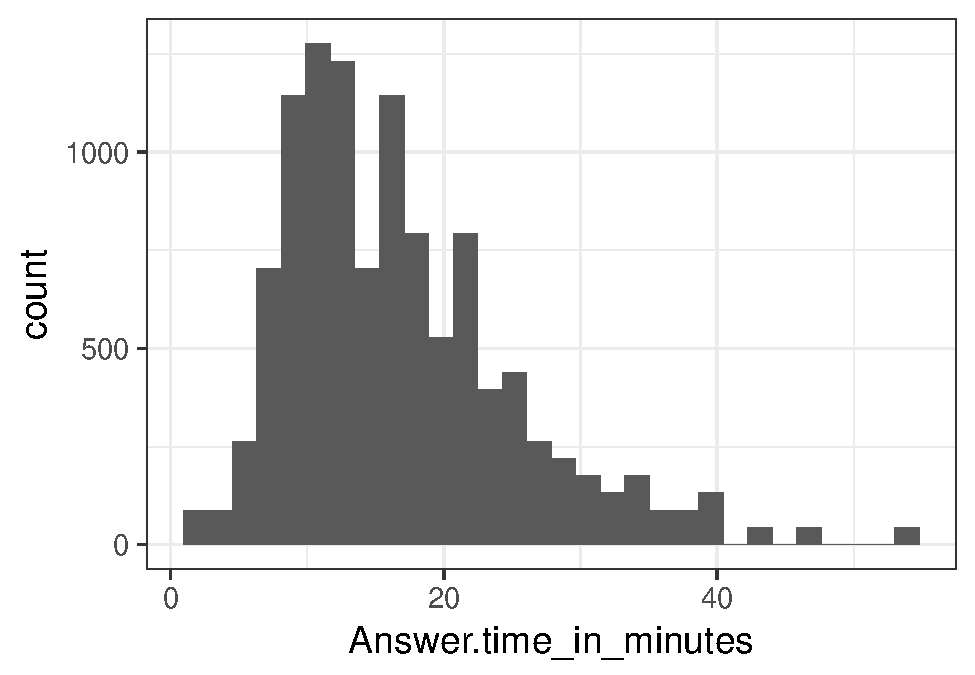
\includegraphics{visualizations_files/figure-latex/unnamed-chunk-6-1.pdf}

\begin{enumerate}
\def\labelenumi{\arabic{enumi}.}
\setcounter{enumi}{1}
\tightlist
\item
  Gender breakdown of trial (not by participant)
\end{enumerate}

\begin{Shaded}
\begin{Highlighting}[]
\KeywordTok{ggplot}\NormalTok{(d, }\KeywordTok{aes}\NormalTok{(gender)) }\OperatorTok{+}
\StringTok{   }\KeywordTok{stat_count}\NormalTok{()}
\end{Highlighting}
\end{Shaded}

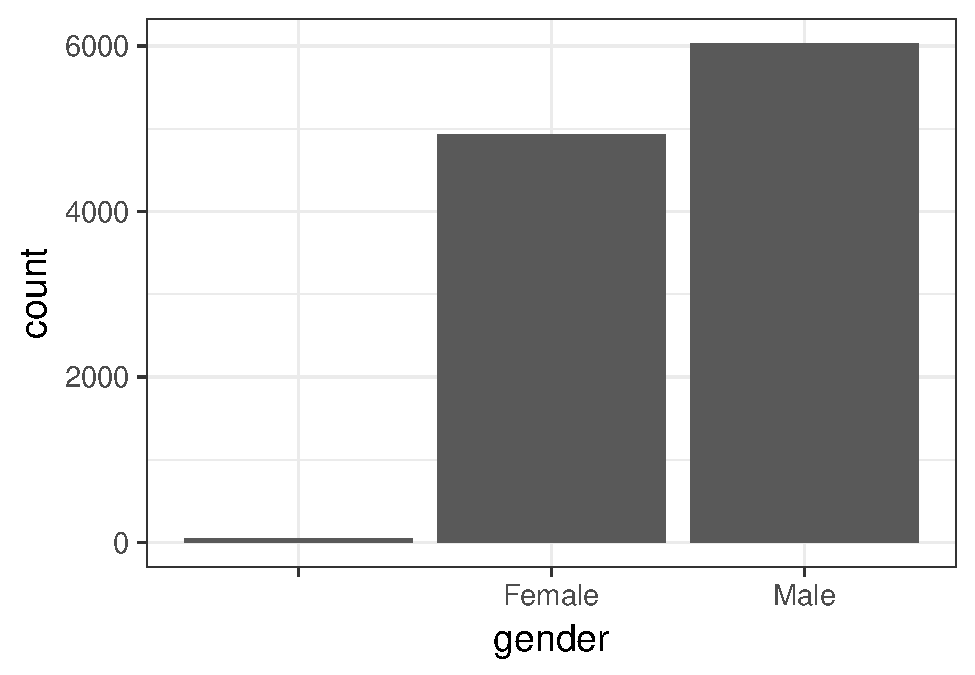
\includegraphics{visualizations_files/figure-latex/unnamed-chunk-7-1.pdf}
3. HIT Understanding

\begin{Shaded}
\begin{Highlighting}[]
\KeywordTok{ggplot}\NormalTok{(d, }\KeywordTok{aes}\NormalTok{(asses)) }\OperatorTok{+}
\StringTok{   }\KeywordTok{stat_count}\NormalTok{()}
\end{Highlighting}
\end{Shaded}

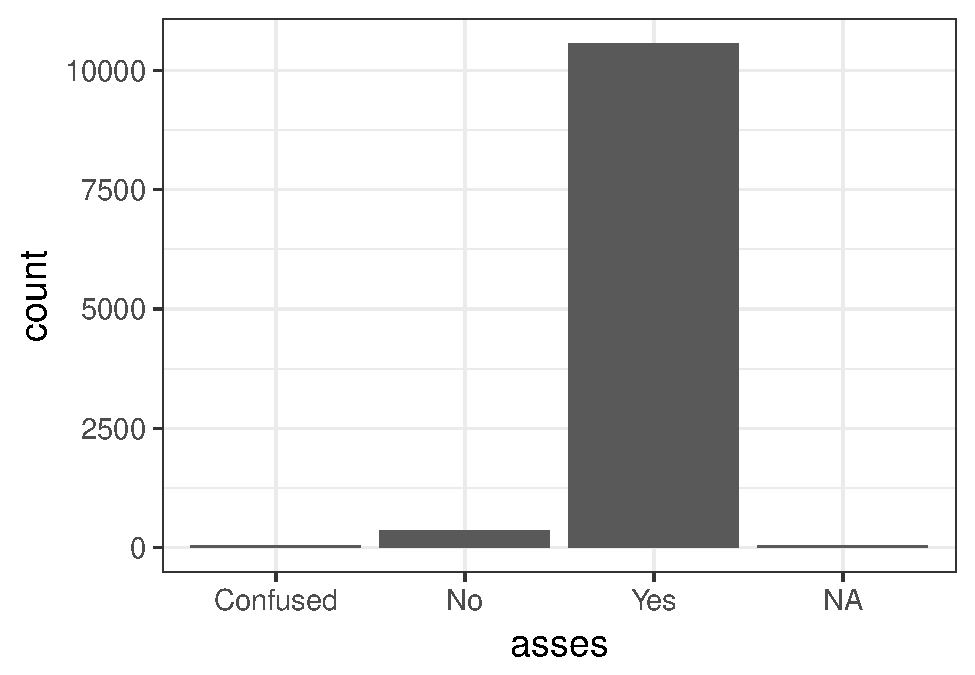
\includegraphics{visualizations_files/figure-latex/unnamed-chunk-8-1.pdf}

\begin{enumerate}
\def\labelenumi{\arabic{enumi}.}
\setcounter{enumi}{3}
\tightlist
\item
  Histogram of age by trial
\end{enumerate}

\begin{Shaded}
\begin{Highlighting}[]
\KeywordTok{ggplot}\NormalTok{(d, }\KeywordTok{aes}\NormalTok{(age)) }\OperatorTok{+}
\StringTok{   }\KeywordTok{geom_histogram}\NormalTok{()}
\end{Highlighting}
\end{Shaded}

\begin{verbatim}
## `stat_bin()` using `bins = 30`. Pick better value with `binwidth`.
\end{verbatim}

\begin{verbatim}
## Warning: Removed 44 rows containing non-finite values (stat_bin).
\end{verbatim}

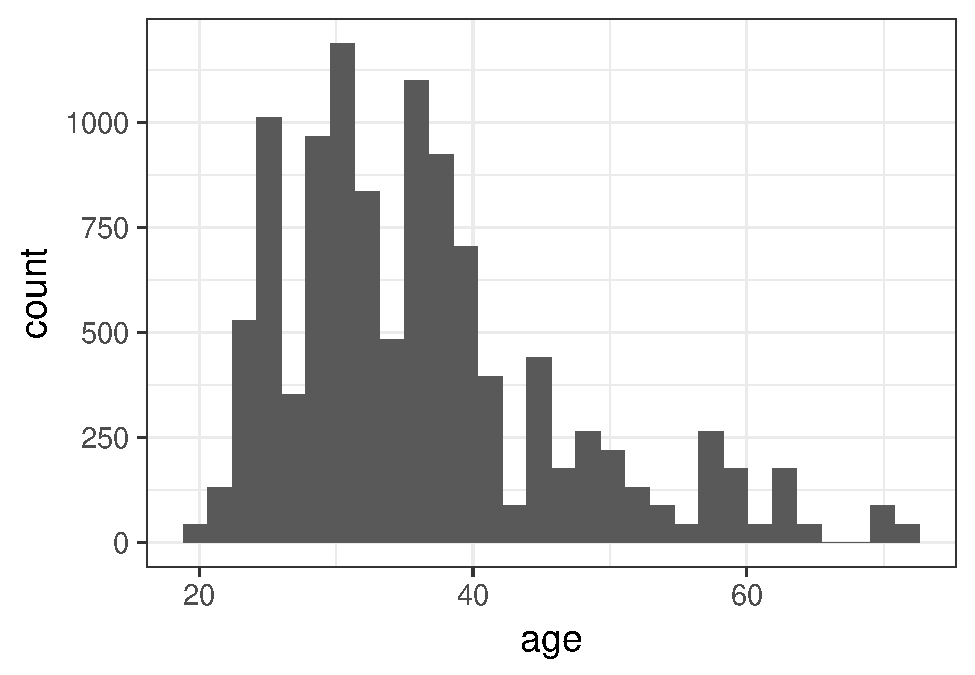
\includegraphics{visualizations_files/figure-latex/unnamed-chunk-9-1.pdf}

\begin{enumerate}
\def\labelenumi{\arabic{enumi}.}
\setcounter{enumi}{4}
\tightlist
\item
  Histogram of education by trial
\end{enumerate}

\begin{Shaded}
\begin{Highlighting}[]
\KeywordTok{ggplot}\NormalTok{(d, }\KeywordTok{aes}\NormalTok{(education)) }\OperatorTok{+}
\StringTok{   }\KeywordTok{stat_count}\NormalTok{()}
\end{Highlighting}
\end{Shaded}

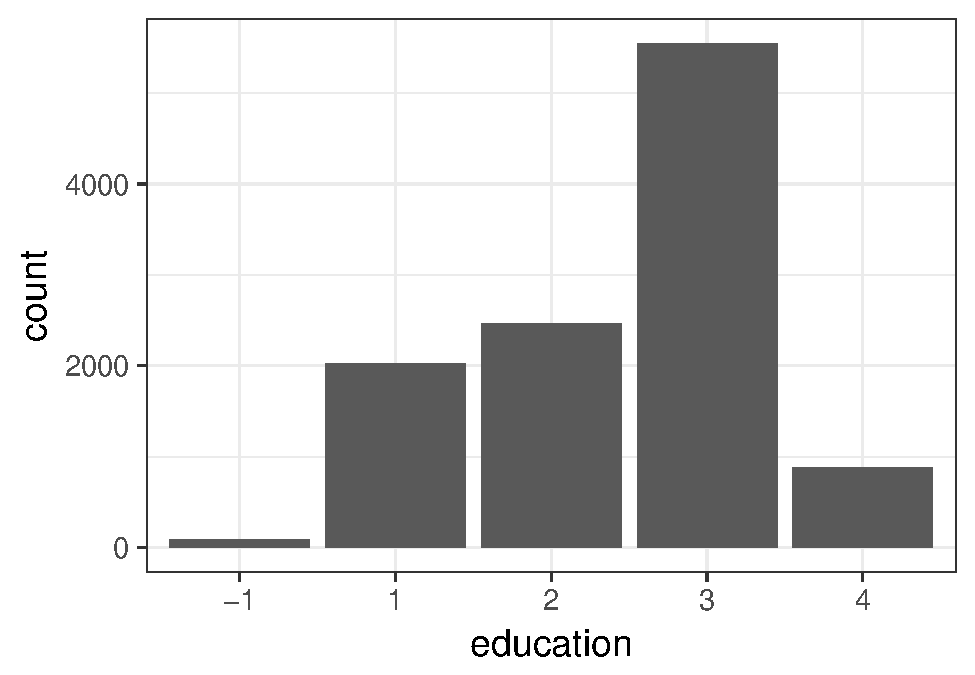
\includegraphics{visualizations_files/figure-latex/unnamed-chunk-10-1.pdf}

\begin{enumerate}
\def\labelenumi{\arabic{enumi}.}
\setcounter{enumi}{5}
\tightlist
\item
  Histogram of language by trial
\end{enumerate}

\begin{Shaded}
\begin{Highlighting}[]
\KeywordTok{ggplot}\NormalTok{(d, }\KeywordTok{aes}\NormalTok{(language)) }\OperatorTok{+}
\StringTok{   }\KeywordTok{stat_count}\NormalTok{() }\OperatorTok{+}
\StringTok{   }\KeywordTok{theme}\NormalTok{(}\DataTypeTok{axis.text.x=}\KeywordTok{element_text}\NormalTok{(}\DataTypeTok{angle=}\DecValTok{45}\NormalTok{,}\DataTypeTok{hjust=}\DecValTok{1}\NormalTok{,}\DataTypeTok{vjust=}\DecValTok{1}\NormalTok{))}
\end{Highlighting}
\end{Shaded}

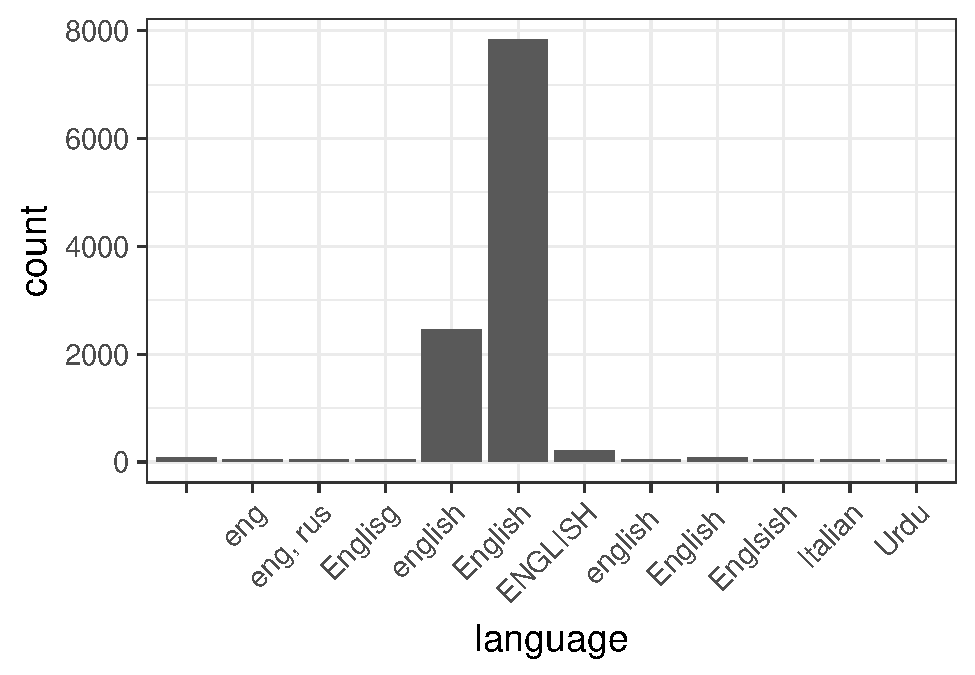
\includegraphics{visualizations_files/figure-latex/unnamed-chunk-11-1.pdf}
7. Histogram of enjoyment by trial

\begin{Shaded}
\begin{Highlighting}[]
\KeywordTok{ggplot}\NormalTok{(d, }\KeywordTok{aes}\NormalTok{(enjoyment)) }\OperatorTok{+}
\StringTok{  }\KeywordTok{stat_count}\NormalTok{()}
\end{Highlighting}
\end{Shaded}

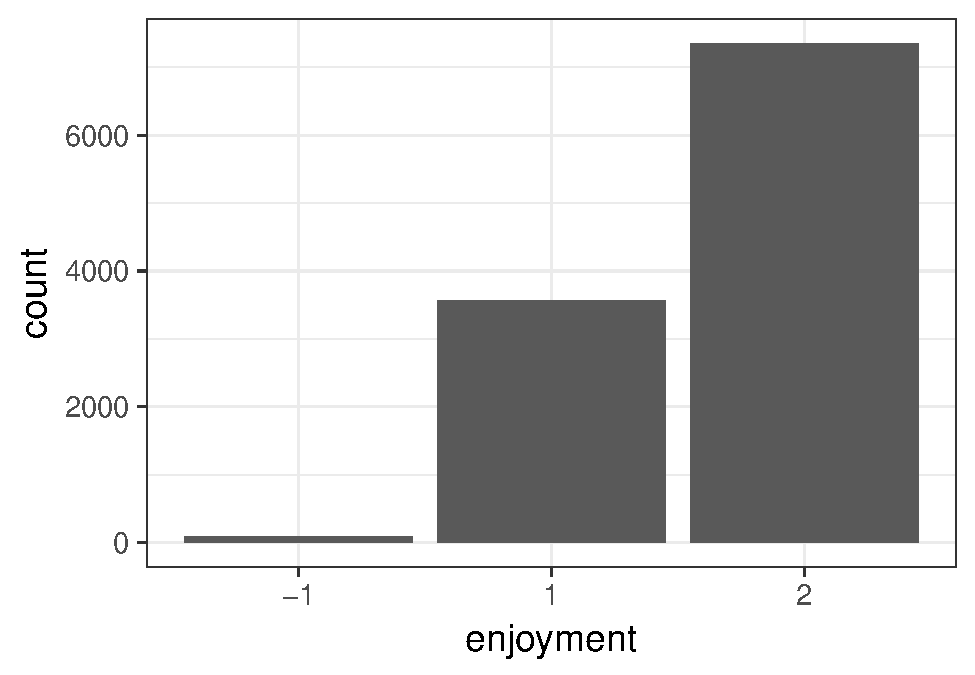
\includegraphics{visualizations_files/figure-latex/unnamed-chunk-12-1.pdf}

\subsection{Part 3: Implementing Exclusion
Criteria}\label{part-3-implementing-exclusion-criteria}

The exclusion criteria for this experiment are as follows: * Exclusion
criterion 0: native language not English * Exclusion criterion 1:
response time more than 2 sd's away from mean completion time *
Exclusion criterion 2: Slider responses not close enough to the
(clearly) correct side in exh block * Exclusion criterion 3: Incorrect
MC response in qud block to 2 attention checks * JD: we need to discuss
the second two exclusion criteria

We excluded 25 participants overall (2 non-native English speaker, 6 on
the basis of time, and 17 on the basis of failing attention checks
during either block of the experiment).

\begin{Shaded}
\begin{Highlighting}[]
\CommentTok{#Finding the failures}
\NormalTok{fails0 =}\StringTok{ }\NormalTok{d }\OperatorTok
\StringTok{  }\KeywordTok{filter}\NormalTok{(language }\OperatorTok{==}\StringTok{ 'Urdu'} \OperatorTok{|}\StringTok{ }\NormalTok{language }\OperatorTok{==}\StringTok{ 'Italian'}\NormalTok{) }\OperatorTok
\StringTok{  }\KeywordTok{droplevels}\NormalTok{()}

\NormalTok{fails1 =}\StringTok{ }\NormalTok{d }\OperatorTok
\StringTok{  }\KeywordTok{filter}\NormalTok{((}\KeywordTok{abs}\NormalTok{(Answer.time_in_minutes}\OperatorTok{-}\KeywordTok{mean}\NormalTok{(d}\OperatorTok{$}\NormalTok{Answer.time_in_minutes)) }\OperatorTok{>}\StringTok{ }\NormalTok{(}\FloatTok{2.5}\OperatorTok{*}\KeywordTok{sd}\NormalTok{(d}\OperatorTok{$}\NormalTok{Answer.time_in_minutes)))) }\OperatorTok\StringTok{ }
\StringTok{  }\KeywordTok{droplevels}\NormalTok{()}

\NormalTok{fails2 =}\StringTok{ }\NormalTok{d }\OperatorTok
\StringTok{  }\KeywordTok{filter}\NormalTok{((block }\OperatorTok{==}\StringTok{ 'exhaustivity'} \OperatorTok{&}\StringTok{ }\NormalTok{trial_type }\OperatorTok{==}\StringTok{ "filler"} \OperatorTok{&}\StringTok{ }\NormalTok{qud }\OperatorTok{==}\StringTok{ "exhaustive"} \OperatorTok{&}\StringTok{ }\KeywordTok{as.numeric}\NormalTok{(}\KeywordTok{as.character}\NormalTok{(response)) }\OperatorTok{<}\StringTok{ }\FloatTok{0.7}\NormalTok{) }\OperatorTok{|}\StringTok{ }\NormalTok{(block }\OperatorTok{==}\StringTok{ 'exhaustivity'} \OperatorTok{&}\StringTok{ }\NormalTok{trial_type }\OperatorTok{==}\StringTok{ "filler"} \OperatorTok{&}\StringTok{ }\NormalTok{qud }\OperatorTok{==}\StringTok{ "polar"} \OperatorTok{&}\StringTok{ }\KeywordTok{as.numeric}\NormalTok{(}\KeywordTok{as.character}\NormalTok{(response)) }\OperatorTok{>}\StringTok{ }\FloatTok{0.25}\NormalTok{)) }\OperatorTok
\StringTok{  }\KeywordTok{droplevels}\NormalTok{()}
\end{Highlighting}
\end{Shaded}

\begin{verbatim}
## Warning in evalq((block == "exhaustivity" & trial_type == "filler" & qud
## == : NAs introduced by coercion

## Warning in evalq((block == "exhaustivity" & trial_type == "filler" & qud
## == : NAs introduced by coercion
\end{verbatim}

\begin{Shaded}
\begin{Highlighting}[]
\NormalTok{fails3 =}\StringTok{ }\NormalTok{d }\OperatorTok\StringTok{ }\KeywordTok{filter}\NormalTok{((block }\OperatorTok{==}\StringTok{ 'qud_assessment'} \OperatorTok{&}\StringTok{ }\NormalTok{trial_type }\OperatorTok{==}\StringTok{ "filler"} \OperatorTok{&}\StringTok{ }\NormalTok{qud }\OperatorTok{==}\StringTok{ "exhaustive"} \OperatorTok{&}\StringTok{ }\NormalTok{response }\OperatorTok{!=}\StringTok{ 'exhaustive'}\NormalTok{) }\OperatorTok{|}\StringTok{ }\NormalTok{(block }\OperatorTok{==}\StringTok{ 'qud_assessment'} \OperatorTok{&}\NormalTok{trial_type }\OperatorTok{==}\StringTok{ "filler"} \OperatorTok{&}\StringTok{ }\NormalTok{qud }\OperatorTok{==}\StringTok{ "polar"} \OperatorTok{&}\StringTok{ }\NormalTok{response }\OperatorTok{!=}\StringTok{ 'polar'}\NormalTok{))}\OperatorTok
\StringTok{ }\KeywordTok{droplevels}\NormalTok{()}

\CommentTok{#Filtering the failures}
\NormalTok{d =}\StringTok{ }\NormalTok{d }\OperatorTok
\StringTok{  }\KeywordTok{filter}\NormalTok{(workerid }\OperatorTok\StringTok{ }\NormalTok{fails0}\OperatorTok{$}\NormalTok{workerid }\OperatorTok{==}\StringTok{ }\OtherTok{FALSE} \OperatorTok{&}\StringTok{ }\NormalTok{workerid }\OperatorTok\StringTok{ }\NormalTok{fails1}\OperatorTok{$}\NormalTok{workerid }\OperatorTok{==}\StringTok{ }\OtherTok{FALSE} \OperatorTok{&}\StringTok{ }\NormalTok{workerid }\OperatorTok\StringTok{ }\NormalTok{fails2}\OperatorTok{$}\NormalTok{workerid }\OperatorTok{==}\StringTok{ }\OtherTok{FALSE} \OperatorTok{&}\StringTok{ }\NormalTok{workerid }\OperatorTok\StringTok{ }\NormalTok{fails3}\OperatorTok{$}\NormalTok{workerid }\OperatorTok{==}\StringTok{ }\OtherTok{FALSE}\NormalTok{) }\OperatorTok
\StringTok{  }\KeywordTok{droplevels}\NormalTok{()}
\end{Highlighting}
\end{Shaded}

\subsection{Part 4: Separating the trials into
block}\label{part-4-separating-the-trials-into-block}

\begin{Shaded}
\begin{Highlighting}[]
\CommentTok{# exhaustivity block critical trials  }
\NormalTok{exhaustivity =}\StringTok{ }\NormalTok{d }\OperatorTok
\StringTok{  }\KeywordTok{filter}\NormalTok{(block }\OperatorTok{==}\StringTok{ 'exhaustivity'}\NormalTok{) }\OperatorTok
\StringTok{  }\KeywordTok{filter}\NormalTok{(trial_type }\OperatorTok{==}\StringTok{ 'critical'}\NormalTok{)}\OperatorTok
\StringTok{  }\KeywordTok{droplevels}\NormalTok{()}

\NormalTok{exhaustivity}\OperatorTok{$}\NormalTok{response =}\StringTok{ }\KeywordTok{as.numeric}\NormalTok{(}\KeywordTok{as.character}\NormalTok{(exhaustivity}\OperatorTok{$}\NormalTok{response))}

\CommentTok{# qud block critical trials only}
\NormalTok{qud =}\StringTok{ }\NormalTok{d }\OperatorTok
\StringTok{  }\KeywordTok{filter}\NormalTok{(block }\OperatorTok{==}\StringTok{ 'qud_assessment'}\NormalTok{) }\OperatorTok
\StringTok{  }\KeywordTok{filter}\NormalTok{(trial_type }\OperatorTok{==}\StringTok{ 'critical'}\NormalTok{)}\OperatorTok
\StringTok{  }\KeywordTok{droplevels}\NormalTok{()}
\end{Highlighting}
\end{Shaded}

\subsection{Part 5: Determining sensitivity score by subject and by
item}\label{part-5-determining-sensitivity-score-by-subject-and-by-item}

In this experiment, sensitivity score (a score that tells how
susceptible slider responses are to contextual QUD manipulation) is
computed by taking the proportion of exhaustive responses to trials
where the context induced an exhaustive QUD and subtracting the
proportion of exhaustive responses to trials where the context induced a
polar QUD.

\begin{Shaded}
\begin{Highlighting}[]
\CommentTok{#Determining by-subject sensitivity score}
\NormalTok{sensitivity =}\StringTok{ }\NormalTok{qud }\OperatorTok\StringTok{ }
\StringTok{  }\KeywordTok{group_by}\NormalTok{(workerid,qud) }\OperatorTok
\StringTok{  }\KeywordTok{summarise}\NormalTok{(}\DataTypeTok{Mean=}\KeywordTok{mean}\NormalTok{(response }\OperatorTok{==}\StringTok{ 'exhaustive'}\NormalTok{)) }\OperatorTok
\StringTok{  }\KeywordTok{spread}\NormalTok{(qud,Mean) }\OperatorTok
\StringTok{  }\KeywordTok{summarise}\NormalTok{(}\DataTypeTok{sensitivityScore =}\NormalTok{ exhaustive }\OperatorTok{-}\StringTok{ }\NormalTok{polar)}

\CommentTok{#Joining by-subject sensitivity score to full datasets}
\NormalTok{qud =}\StringTok{ }\NormalTok{qud }\OperatorTok
\StringTok{  }\KeywordTok{right_join}\NormalTok{(sensitivity, }\DataTypeTok{by=}\KeywordTok{c}\NormalTok{(}\StringTok{'workerid'}\NormalTok{))}

\NormalTok{exhaustivity =}\StringTok{ }\NormalTok{exhaustivity }\OperatorTok
\StringTok{  }\KeywordTok{right_join}\NormalTok{(sensitivity, }\DataTypeTok{by=}\KeywordTok{c}\NormalTok{(}\StringTok{'workerid'}\NormalTok{))}

\CommentTok{#Determining something's QUD sensitivity score:}
\NormalTok{sensitivityItem =}\StringTok{ }\NormalTok{qud }\OperatorTok\StringTok{ }
\StringTok{  }\KeywordTok{group_by}\NormalTok{(topic,qud) }\OperatorTok
\StringTok{  }\KeywordTok{summarise}\NormalTok{(}\DataTypeTok{Mean=}\KeywordTok{mean}\NormalTok{(response }\OperatorTok{==}\StringTok{ 'exhaustive'}\NormalTok{)) }\OperatorTok
\StringTok{  }\KeywordTok{spread}\NormalTok{(qud,Mean) }\OperatorTok
\StringTok{  }\KeywordTok{summarise}\NormalTok{(}\DataTypeTok{sensitivityScoreItem =}\NormalTok{ exhaustive }\OperatorTok{-}\StringTok{ }\NormalTok{polar)}
\end{Highlighting}
\end{Shaded}

\begin{enumerate}
\def\labelenumi{\arabic{enumi}.}
\setcounter{enumi}{7}
\tightlist
\item
  Plotting a histogram of participant sensitivity
\end{enumerate}

\begin{Shaded}
\begin{Highlighting}[]
\KeywordTok{ggplot}\NormalTok{(sensitivity, }\KeywordTok{aes}\NormalTok{(}\DataTypeTok{x=}\NormalTok{sensitivityScore)) }\OperatorTok{+}
\StringTok{  }\KeywordTok{geom_histogram}\NormalTok{()}
\end{Highlighting}
\end{Shaded}

\begin{verbatim}
## `stat_bin()` using `bins = 30`. Pick better value with `binwidth`.
\end{verbatim}

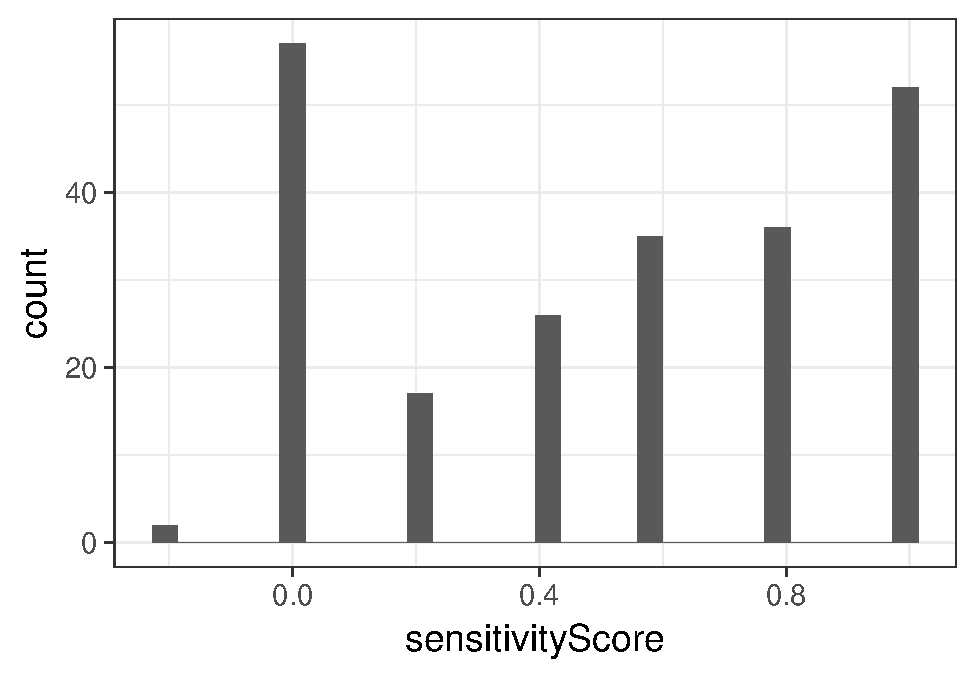
\includegraphics{visualizations_files/figure-latex/unnamed-chunk-16-1.pdf}

\subsection{Part 6: Determining mean prior belief by item and
integrating into experimental
data}\label{part-6-determining-mean-prior-belief-by-item-and-integrating-into-experimental-data}

\begin{Shaded}
\begin{Highlighting}[]
\CommentTok{#Getting mean priors over all items and adding their "topic" value}
\NormalTok{priorsItems =}\StringTok{ }\NormalTok{priors }\OperatorTok
\StringTok{  }\KeywordTok{group_by}\NormalTok{(scenario) }\OperatorTok
\StringTok{  }\KeywordTok{summarise}\NormalTok{(}\DataTypeTok{Mean=}\KeywordTok{mean}\NormalTok{(response),}\DataTypeTok{CILow=}\KeywordTok{ci.low}\NormalTok{(response),}\DataTypeTok{CIHigh=}\KeywordTok{ci.high}\NormalTok{(response)) }\OperatorTok
\StringTok{  }\KeywordTok{ungroup}\NormalTok{() }\OperatorTok
\StringTok{  }\KeywordTok{mutate}\NormalTok{(}\DataTypeTok{YMin=}\NormalTok{Mean}\OperatorTok{-}\NormalTok{CILow,}\DataTypeTok{YMax=}\NormalTok{Mean}\OperatorTok{+}\NormalTok{CIHigh) }\OperatorTok
\StringTok{  }\KeywordTok{mutate}\NormalTok{(}\DataTypeTok{Mean_Prior =}\NormalTok{ Mean,}\DataTypeTok{YMin_Prior =}\NormalTok{ YMin, }\DataTypeTok{YMax_Prior =}\NormalTok{ YMax) }\OperatorTok
\StringTok{  }\KeywordTok{mutate}\NormalTok{(}\DataTypeTok{Scenario =} \KeywordTok{fct_reorder}\NormalTok{(scenario,Mean)) }\OperatorTok
\StringTok{  }\KeywordTok{arrange}\NormalTok{(}\KeywordTok{desc}\NormalTok{(Scenario)) }\OperatorTok
\StringTok{  }\KeywordTok{cbind}\NormalTok{(}\KeywordTok{data.frame}\NormalTok{(}\DataTypeTok{topic =} \KeywordTok{c}\NormalTok{(}\StringTok{'bell peppers'}\NormalTok{,}\StringTok{'tomatoes'}\NormalTok{,}\StringTok{'salad'}\NormalTok{,}\StringTok{'kale'}\NormalTok{,}\StringTok{'salmon'}\NormalTok{,}\StringTok{'notUsed'}\NormalTok{,}\StringTok{'lipstick'}\NormalTok{,}\StringTok{'sandals'}\NormalTok{,}\StringTok{'notUsed'}\NormalTok{,}\StringTok{'weights'}\NormalTok{,}\StringTok{'notUsed'}\NormalTok{,}\StringTok{'freestyle'}\NormalTok{,}\StringTok{'tulips'}\NormalTok{,}\StringTok{'gas station'}\NormalTok{,}\StringTok{'notUsed'}\NormalTok{,}\StringTok{'ballad'}\NormalTok{,}\StringTok{'fruit basket'}\NormalTok{,}\StringTok{'notUsed'}\NormalTok{,}\StringTok{'perfume'}\NormalTok{,}\StringTok{'gym'}\NormalTok{,}\StringTok{'cereal'}\NormalTok{,}\StringTok{'partner'}\NormalTok{,}\StringTok{'San Francisco'}\NormalTok{,}\StringTok{'pottery'}\NormalTok{,}\StringTok{'ice cream'}\NormalTok{)))}

\CommentTok{#Making sure topic value is a factor}
\NormalTok{priorsItems}\OperatorTok{$}\NormalTok{topic =}\StringTok{ }\KeywordTok{as.factor}\NormalTok{(}\KeywordTok{as.character}\NormalTok{(priorsItems}\OperatorTok{$}\NormalTok{topic))}

\CommentTok{#Integrating priors with data }
\NormalTok{exhaustivity =}\StringTok{ }\NormalTok{exhaustivity }\OperatorTok
\StringTok{  }\KeywordTok{left_join}\NormalTok{(priorsItems,}\DataTypeTok{by=}\KeywordTok{c}\NormalTok{(}\StringTok{'topic'}\NormalTok{))}
\end{Highlighting}
\end{Shaded}

\begin{verbatim}
## Warning: Column `topic` joining factors with different levels, coercing to
## character vector
\end{verbatim}

\subsection{Part 7: Critical
visualizations}\label{part-7-critical-visualizations}

\begin{enumerate}
\def\labelenumi{\arabic{enumi}.}
\setcounter{enumi}{8}
\tightlist
\item
  Mean slider response (from exhaustivity block) in polar and exhaustive
  QUD conditions
\end{enumerate}

\begin{Shaded}
\begin{Highlighting}[]
\NormalTok{means =}\StringTok{ }\NormalTok{exhaustivity }\OperatorTok
\StringTok{  }\KeywordTok{group_by}\NormalTok{(qud) }\OperatorTok
\StringTok{  }\KeywordTok{summarise}\NormalTok{(}\DataTypeTok{Mean=}\KeywordTok{mean}\NormalTok{(response),}\DataTypeTok{CILow=}\KeywordTok{ci.low}\NormalTok{(response),}\DataTypeTok{CIHigh=}\KeywordTok{ci.high}\NormalTok{(response)) }\OperatorTok
\StringTok{  }\KeywordTok{ungroup}\NormalTok{() }\OperatorTok
\StringTok{  }\KeywordTok{mutate}\NormalTok{(}\DataTypeTok{YMin=}\NormalTok{Mean}\OperatorTok{-}\NormalTok{CILow,}\DataTypeTok{YMax=}\NormalTok{Mean}\OperatorTok{+}\NormalTok{CIHigh) }\OperatorTok
\StringTok{  }\KeywordTok{mutate}\NormalTok{(}\DataTypeTok{Mean_New =}\NormalTok{ Mean,}\DataTypeTok{YMin_New =}\NormalTok{ YMin, }\DataTypeTok{YMax_New =}\NormalTok{ YMax) }\OperatorTok
\StringTok{  }\KeywordTok{mutate}\NormalTok{(}\DataTypeTok{Qud =} \KeywordTok{fct_reorder}\NormalTok{(qud,Mean))}

\NormalTok{means_subj =}\StringTok{ }\NormalTok{exhaustivity }\OperatorTok
\StringTok{  }\KeywordTok{group_by}\NormalTok{(qud,workerid) }\OperatorTok
\StringTok{  }\KeywordTok{summarise}\NormalTok{(}\DataTypeTok{Mean=}\KeywordTok{mean}\NormalTok{(response),}\DataTypeTok{CILow=}\KeywordTok{ci.low}\NormalTok{(response),}\DataTypeTok{CIHigh=}\KeywordTok{ci.high}\NormalTok{(response)) }\OperatorTok
\StringTok{  }\KeywordTok{ungroup}\NormalTok{() }\OperatorTok
\StringTok{  }\KeywordTok{mutate}\NormalTok{(}\DataTypeTok{YMin=}\NormalTok{Mean}\OperatorTok{-}\NormalTok{CILow,}\DataTypeTok{YMax=}\NormalTok{Mean}\OperatorTok{+}\NormalTok{CIHigh) }\OperatorTok
\StringTok{  }\KeywordTok{mutate}\NormalTok{(}\DataTypeTok{Mean_New =}\NormalTok{ Mean,}\DataTypeTok{YMin_New =}\NormalTok{ YMin, }\DataTypeTok{YMax_New =}\NormalTok{ YMax) }\OperatorTok
\StringTok{  }\KeywordTok{mutate}\NormalTok{(}\DataTypeTok{Qud =} \KeywordTok{fct_reorder}\NormalTok{(qud,Mean))}

\CommentTok{#plot of mean slider response (with error bars) per QUD}
\KeywordTok{ggplot}\NormalTok{(means, }\KeywordTok{aes}\NormalTok{(}\DataTypeTok{x=}\NormalTok{qud,}\DataTypeTok{y=}\NormalTok{Mean)) }\OperatorTok{+}
\StringTok{  }\KeywordTok{geom_bar}\NormalTok{(}\DataTypeTok{stat=}\StringTok{"identity"}\NormalTok{) }\OperatorTok{+}
\StringTok{  }\KeywordTok{geom_line}\NormalTok{(}\DataTypeTok{data=}\NormalTok{means_subj,}\KeywordTok{aes}\NormalTok{(}\DataTypeTok{group=}\NormalTok{workerid),}\DataTypeTok{alpha=}\NormalTok{.}\DecValTok{5}\NormalTok{,}\DataTypeTok{color=}\StringTok{"gray60"}\NormalTok{) }\OperatorTok{+}
\StringTok{  }\KeywordTok{geom_errorbar}\NormalTok{(}\KeywordTok{aes}\NormalTok{(}\DataTypeTok{ymin=}\NormalTok{YMin,}\DataTypeTok{ymax=}\NormalTok{YMax),}\DataTypeTok{width=}\NormalTok{.}\DecValTok{25}\NormalTok{) }\OperatorTok{+}
\StringTok{  }\KeywordTok{theme}\NormalTok{(}\DataTypeTok{axis.text.x=}\KeywordTok{element_text}\NormalTok{(}\DataTypeTok{angle=}\DecValTok{45}\NormalTok{,}\DataTypeTok{hjust=}\DecValTok{1}\NormalTok{,}\DataTypeTok{vjust=}\DecValTok{1}\NormalTok{))}
\end{Highlighting}
\end{Shaded}

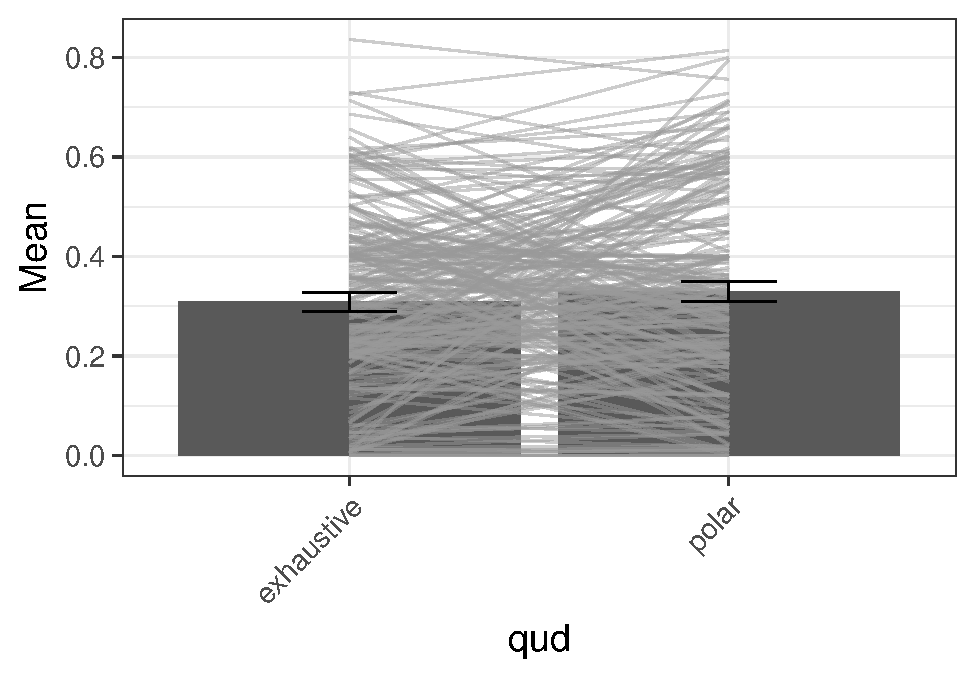
\includegraphics{visualizations_files/figure-latex/unnamed-chunk-18-1.pdf}

\begin{Shaded}
\begin{Highlighting}[]
\CommentTok{#plot of mean slider response (with error bars) per QUD per subject}
\KeywordTok{ggplot}\NormalTok{(means_subj, }\KeywordTok{aes}\NormalTok{(}\DataTypeTok{x=}\NormalTok{qud,}\DataTypeTok{y=}\NormalTok{Mean)) }\OperatorTok{+}
\StringTok{  }\KeywordTok{geom_bar}\NormalTok{(}\DataTypeTok{stat=}\StringTok{"identity"}\NormalTok{) }\OperatorTok{+}
\StringTok{  }\KeywordTok{facet_wrap}\NormalTok{(}\OperatorTok{~}\NormalTok{workerid) }\OperatorTok{+}
\StringTok{  }\CommentTok{#geom_line(data=means_subj,aes(group=workerid),alpha=.5,color="gray60") +}
\StringTok{  }\KeywordTok{geom_errorbar}\NormalTok{(}\KeywordTok{aes}\NormalTok{(}\DataTypeTok{ymin=}\NormalTok{YMin,}\DataTypeTok{ymax=}\NormalTok{YMax),}\DataTypeTok{width=}\NormalTok{.}\DecValTok{25}\NormalTok{) }\OperatorTok{+}
\StringTok{  }\KeywordTok{theme}\NormalTok{(}\DataTypeTok{axis.text.x=}\KeywordTok{element_text}\NormalTok{(}\DataTypeTok{angle=}\DecValTok{45}\NormalTok{,}\DataTypeTok{hjust=}\DecValTok{1}\NormalTok{,}\DataTypeTok{vjust=}\DecValTok{1}\NormalTok{))}
\end{Highlighting}
\end{Shaded}

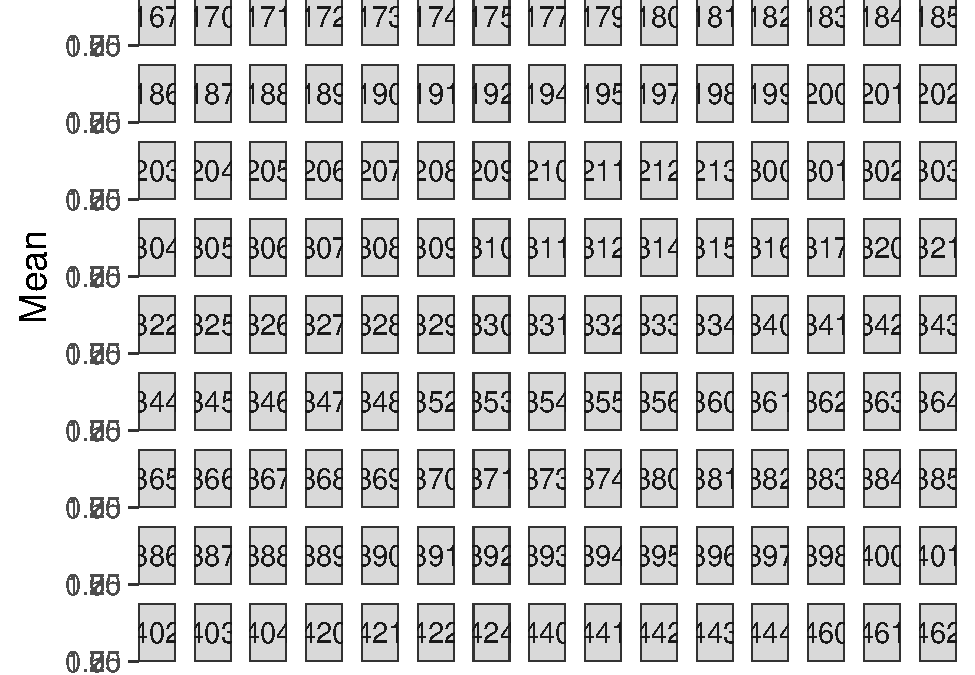
\includegraphics{visualizations_files/figure-latex/unnamed-chunk-18-2.pdf}

\begin{enumerate}
\def\labelenumi{\arabic{enumi}.}
\setcounter{enumi}{9}
\tightlist
\item
  Proportion of exhaustive responses (from QUD assessment block) in the
  polar and exhaustive QUD conditions, by item as a histogram
\end{enumerate}

\begin{Shaded}
\begin{Highlighting}[]
\CommentTok{#Compute proportions of exhaustive responses by qud}
\NormalTok{cont_qud =}\StringTok{ }\NormalTok{qud }\OperatorTok
\StringTok{  }\KeywordTok{group_by}\NormalTok{(topic,qud) }\OperatorTok
\StringTok{  }\KeywordTok{summarise}\NormalTok{(}\DataTypeTok{ProportionExhaustive =} \KeywordTok{mean}\NormalTok{(response }\OperatorTok{==}\StringTok{ 'exhaustive'}\NormalTok{)) }\OperatorTok
\StringTok{  }\KeywordTok{ungroup}\NormalTok{()}

\KeywordTok{ggplot}\NormalTok{(cont_qud,}\KeywordTok{aes}\NormalTok{(}\DataTypeTok{x=}\NormalTok{ProportionExhaustive,}\DataTypeTok{fill=}\NormalTok{qud))  }\OperatorTok{+}
\StringTok{  }\KeywordTok{geom_histogram}\NormalTok{(}\DataTypeTok{position=}\StringTok{"identity"}\NormalTok{,}\DataTypeTok{alpha=}\NormalTok{.}\DecValTok{5}\NormalTok{)}
\end{Highlighting}
\end{Shaded}

\begin{verbatim}
## `stat_bin()` using `bins = 30`. Pick better value with `binwidth`.
\end{verbatim}

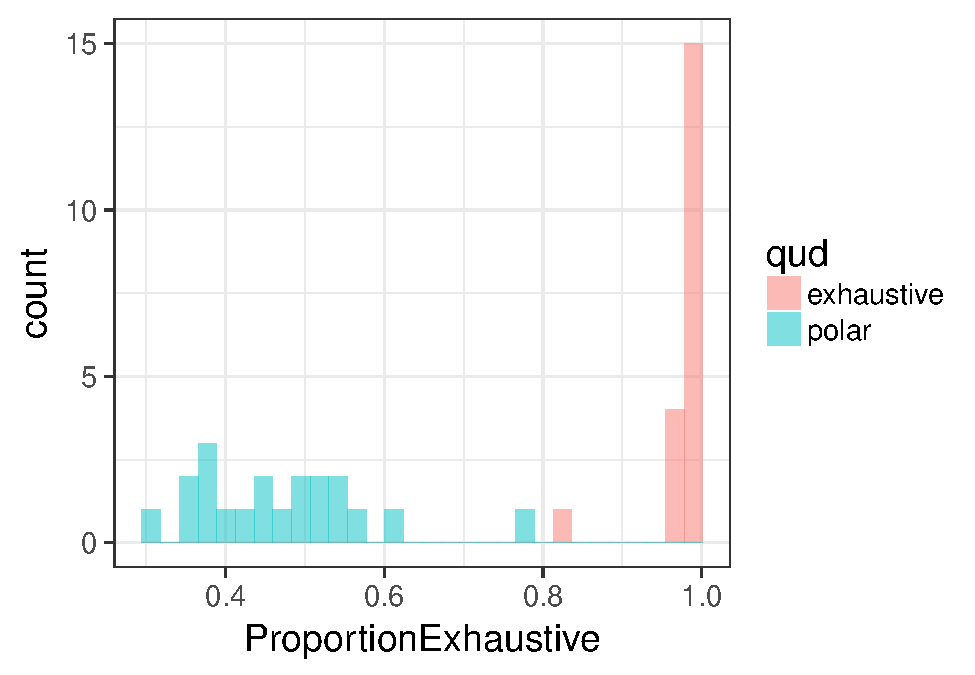
\includegraphics{visualizations_files/figure-latex/unnamed-chunk-19-1.pdf}

\begin{enumerate}
\def\labelenumi{\arabic{enumi}.}
\setcounter{enumi}{10}
\tightlist
\item
  Proportion of exhaustive responses (from QUD assessment block) in the
  polar and exhaustive QUD conditions, by item as a scatterplot
\end{enumerate}

\begin{Shaded}
\begin{Highlighting}[]
\CommentTok{# merge back into exhaustivity}
\NormalTok{exhaustivity =}\StringTok{ }\KeywordTok{left_join}\NormalTok{(exhaustivity,cont_qud,}\DataTypeTok{by=}\KeywordTok{c}\NormalTok{(}\StringTok{"topic"}\NormalTok{,}\StringTok{"qud"}\NormalTok{))}
\end{Highlighting}
\end{Shaded}

\begin{verbatim}
## Warning: Column `topic` joining character vector and factor, coercing into
## character vector
\end{verbatim}

\begin{Shaded}
\begin{Highlighting}[]
\NormalTok{means =}\StringTok{ }\NormalTok{exhaustivity }\OperatorTok
\StringTok{  }\KeywordTok{group_by}\NormalTok{(ProportionExhaustive,qud) }\OperatorTok
\StringTok{  }\KeywordTok{summarise}\NormalTok{(}\DataTypeTok{Mean=}\KeywordTok{mean}\NormalTok{(response),}\DataTypeTok{CILow=}\KeywordTok{ci.low}\NormalTok{(response),}\DataTypeTok{CIHigh=}\KeywordTok{ci.high}\NormalTok{(response))}\OperatorTok
\StringTok{  }\KeywordTok{ungroup}\NormalTok{() }\OperatorTok
\StringTok{  }\KeywordTok{mutate}\NormalTok{(}\DataTypeTok{YMin=}\NormalTok{Mean}\OperatorTok{-}\NormalTok{CILow,}\DataTypeTok{YMax=}\NormalTok{Mean}\OperatorTok{+}\NormalTok{CIHigh)}

\KeywordTok{ggplot}\NormalTok{(means,}\KeywordTok{aes}\NormalTok{(}\DataTypeTok{x=}\NormalTok{ProportionExhaustive,}\DataTypeTok{y=}\NormalTok{Mean,}\DataTypeTok{color=}\NormalTok{qud)) }\OperatorTok{+}
\StringTok{  }\KeywordTok{geom_point}\NormalTok{() }\OperatorTok{+}
\StringTok{  }\KeywordTok{geom_smooth}\NormalTok{(}\DataTypeTok{method=}\StringTok{"lm"}\NormalTok{)}
\end{Highlighting}
\end{Shaded}

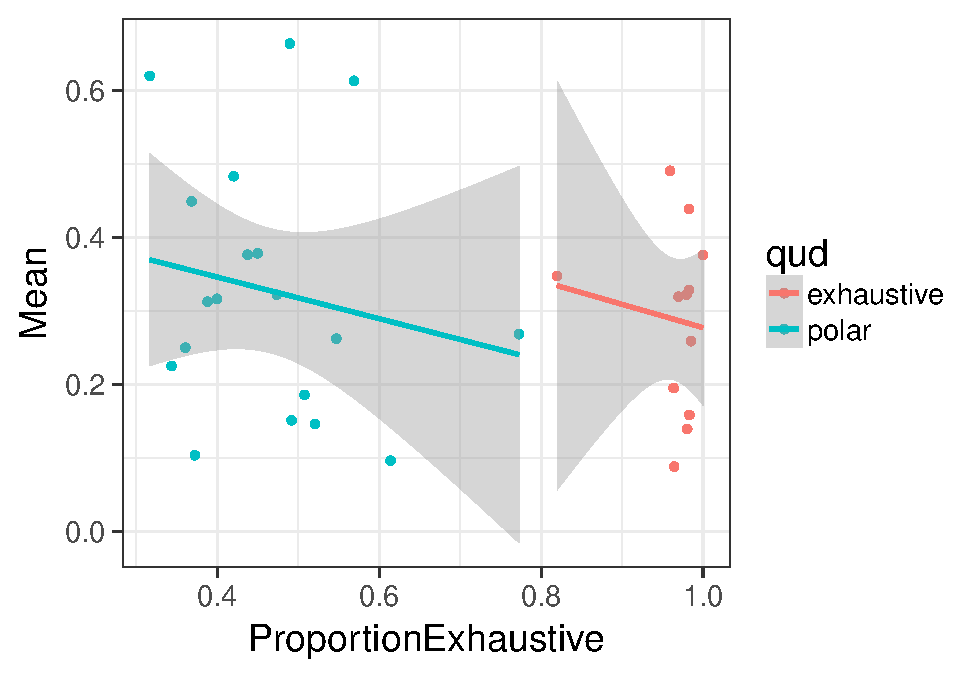
\includegraphics{visualizations_files/figure-latex/unnamed-chunk-20-1.pdf}

\begin{Shaded}
\begin{Highlighting}[]
\CommentTok{#ggsave(file="../graphs/1_critical/mean_slider_line.png")}
\end{Highlighting}
\end{Shaded}

Mean proportion of exhaustive responses in polar versus exhaustive QUD,
as a bar plot

\begin{Shaded}
\begin{Highlighting}[]
\CommentTok{#2. Mean proportion of "exhaustive" responses in the polar versus exhaustive QUD (from qud block)}
\NormalTok{meanExhaustive =}\StringTok{ }\NormalTok{qud }\OperatorTok
\StringTok{  }\KeywordTok{group_by}\NormalTok{(qud)}\OperatorTok
\StringTok{  }\KeywordTok{summarise}\NormalTok{(}\DataTypeTok{Proportion =} \KeywordTok{mean}\NormalTok{(response }\OperatorTok{==}\StringTok{ 'exhaustive'}\NormalTok{),}\DataTypeTok{CILow=}\KeywordTok{ci.low}\NormalTok{(response }\OperatorTok{==}\StringTok{ 'exhaustive'}\NormalTok{),}\DataTypeTok{CIHigh=}\KeywordTok{ci.high}\NormalTok{(response }\OperatorTok{==}\StringTok{ 'exhaustive'}\NormalTok{))}\OperatorTok
\StringTok{  }\KeywordTok{ungroup}\NormalTok{() }\OperatorTok
\StringTok{  }\KeywordTok{mutate}\NormalTok{(}\DataTypeTok{YMin=}\NormalTok{Proportion}\OperatorTok{-}\NormalTok{CILow,}\DataTypeTok{YMax=}\NormalTok{Proportion}\OperatorTok{+}\NormalTok{CIHigh) }\OperatorTok
\StringTok{  }\KeywordTok{mutate}\NormalTok{(}\DataTypeTok{Proportion_New =}\NormalTok{ Proportion,}\DataTypeTok{YMin_New =}\NormalTok{ YMin, }\DataTypeTok{YMax_New =}\NormalTok{ YMax) }\OperatorTok
\StringTok{  }\KeywordTok{mutate}\NormalTok{(}\DataTypeTok{Qud =} \KeywordTok{fct_reorder}\NormalTok{(qud,Proportion))}

\KeywordTok{ggplot}\NormalTok{(meanExhaustive, }\KeywordTok{aes}\NormalTok{(}\DataTypeTok{x=}\NormalTok{Qud,}\DataTypeTok{y=}\NormalTok{Proportion)) }\OperatorTok{+}
\StringTok{  }\KeywordTok{geom_bar}\NormalTok{(}\DataTypeTok{stat=}\StringTok{"identity"}\NormalTok{) }\OperatorTok{+}
\StringTok{  }\KeywordTok{geom_errorbar}\NormalTok{(}\KeywordTok{aes}\NormalTok{(}\DataTypeTok{ymin=}\NormalTok{YMin,}\DataTypeTok{ymax=}\NormalTok{YMax),}\DataTypeTok{width=}\NormalTok{.}\DecValTok{25}\NormalTok{) }\OperatorTok{+}
\StringTok{  }\KeywordTok{theme}\NormalTok{(}\DataTypeTok{axis.text.x=}\KeywordTok{element_text}\NormalTok{(}\DataTypeTok{angle=}\DecValTok{45}\NormalTok{,}\DataTypeTok{hjust=}\DecValTok{1}\NormalTok{,}\DataTypeTok{vjust=}\DecValTok{1}\NormalTok{))}
\end{Highlighting}
\end{Shaded}

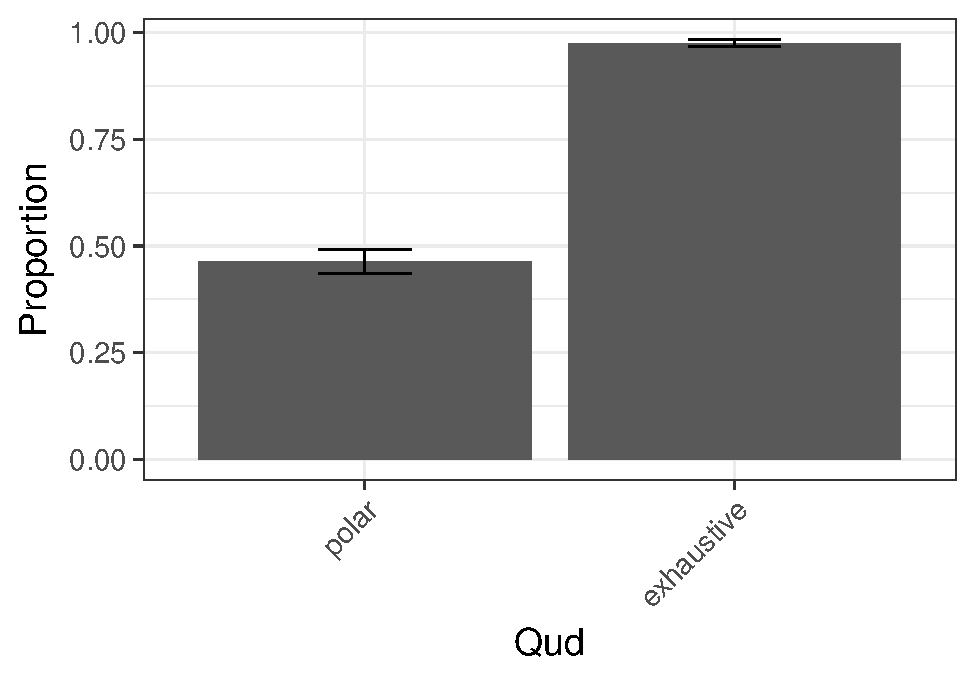
\includegraphics{visualizations_files/figure-latex/unnamed-chunk-21-1.pdf}

\begin{enumerate}
\def\labelenumi{\arabic{enumi}.}
\setcounter{enumi}{11}
\tightlist
\item
  Mean proportion of ``exhaustive'' responses in polar versus exhaustive
  QUD, by subject
\end{enumerate}

\begin{Shaded}
\begin{Highlighting}[]
\NormalTok{meanExhaustive =}\StringTok{ }\NormalTok{qud }\OperatorTok
\StringTok{  }\KeywordTok{group_by}\NormalTok{(qud,workerid)}\OperatorTok
\StringTok{  }\KeywordTok{summarise}\NormalTok{(}\DataTypeTok{Proportion =} \KeywordTok{mean}\NormalTok{(response }\OperatorTok{==}\StringTok{ 'exhaustive'}\NormalTok{),}\DataTypeTok{CILow=}\KeywordTok{ci.low}\NormalTok{(response }\OperatorTok{==}\StringTok{ 'exhaustive'}\NormalTok{),}\DataTypeTok{CIHigh=}\KeywordTok{ci.high}\NormalTok{(response }\OperatorTok{==}\StringTok{ 'exhaustive'}\NormalTok{))}\OperatorTok
\StringTok{  }\KeywordTok{ungroup}\NormalTok{() }\OperatorTok
\StringTok{  }\KeywordTok{mutate}\NormalTok{(}\DataTypeTok{YMin=}\NormalTok{Proportion}\OperatorTok{-}\NormalTok{CILow,}\DataTypeTok{YMax=}\NormalTok{Proportion}\OperatorTok{+}\NormalTok{CIHigh) }\OperatorTok
\StringTok{  }\KeywordTok{mutate}\NormalTok{(}\DataTypeTok{Proportion_New =}\NormalTok{ Proportion,}\DataTypeTok{YMin_New =}\NormalTok{ YMin, }\DataTypeTok{YMax_New =}\NormalTok{ YMax) }\OperatorTok
\StringTok{  }\KeywordTok{mutate}\NormalTok{(}\DataTypeTok{Qud =} \KeywordTok{fct_reorder}\NormalTok{(qud,Proportion))}

\KeywordTok{ggplot}\NormalTok{(meanExhaustive, }\KeywordTok{aes}\NormalTok{(}\DataTypeTok{x=}\NormalTok{Qud,}\DataTypeTok{y=}\NormalTok{Proportion)) }\OperatorTok{+}
\StringTok{  }\KeywordTok{geom_bar}\NormalTok{(}\DataTypeTok{stat=}\StringTok{"identity"}\NormalTok{) }\OperatorTok{+}
\StringTok{  }\KeywordTok{facet_wrap}\NormalTok{(}\OperatorTok{~}\NormalTok{workerid) }\OperatorTok{+}
\StringTok{  }\KeywordTok{geom_errorbar}\NormalTok{(}\KeywordTok{aes}\NormalTok{(}\DataTypeTok{ymin=}\NormalTok{YMin,}\DataTypeTok{ymax=}\NormalTok{YMax),}\DataTypeTok{width=}\NormalTok{.}\DecValTok{25}\NormalTok{) }\OperatorTok{+}
\StringTok{  }\KeywordTok{theme}\NormalTok{(}\DataTypeTok{axis.text.x=}\KeywordTok{element_text}\NormalTok{(}\DataTypeTok{angle=}\DecValTok{45}\NormalTok{,}\DataTypeTok{hjust=}\DecValTok{1}\NormalTok{,}\DataTypeTok{vjust=}\DecValTok{1}\NormalTok{))}
\end{Highlighting}
\end{Shaded}

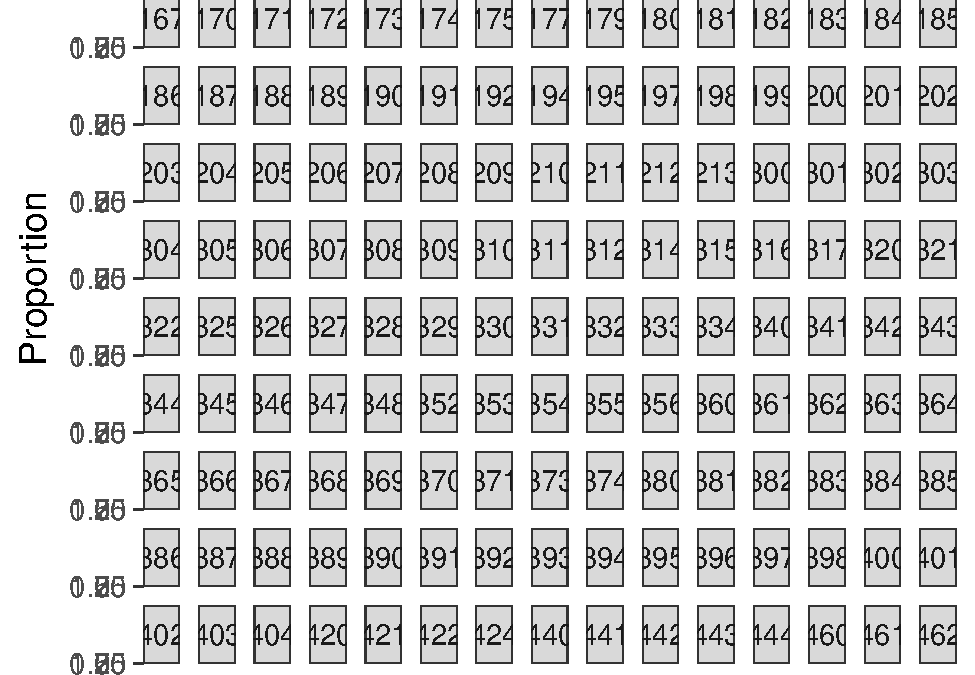
\includegraphics{visualizations_files/figure-latex/unnamed-chunk-22-1.pdf}

\begin{enumerate}
\def\labelenumi{\arabic{enumi}.}
\setcounter{enumi}{12}
\tightlist
\item
  Mean proportion of ``exhaustive'' responses in polar versus exhaustive
  QUD, by item
\end{enumerate}

\begin{Shaded}
\begin{Highlighting}[]
\NormalTok{meanExhaustive =}\StringTok{ }\NormalTok{qud }\OperatorTok
\StringTok{  }\KeywordTok{group_by}\NormalTok{(qud,topic)}\OperatorTok
\StringTok{  }\KeywordTok{summarise}\NormalTok{(}\DataTypeTok{Proportion =} \KeywordTok{mean}\NormalTok{(response }\OperatorTok{==}\StringTok{ 'exhaustive'}\NormalTok{),}\DataTypeTok{CILow=}\KeywordTok{ci.low}\NormalTok{(response }\OperatorTok{==}\StringTok{ 'exhaustive'}\NormalTok{),}\DataTypeTok{CIHigh=}\KeywordTok{ci.high}\NormalTok{(response }\OperatorTok{==}\StringTok{ 'exhaustive'}\NormalTok{))}\OperatorTok
\StringTok{  }\KeywordTok{ungroup}\NormalTok{() }\OperatorTok
\StringTok{  }\KeywordTok{mutate}\NormalTok{(}\DataTypeTok{YMin=}\NormalTok{Proportion}\OperatorTok{-}\NormalTok{CILow,}\DataTypeTok{YMax=}\NormalTok{Proportion}\OperatorTok{+}\NormalTok{CIHigh) }\OperatorTok
\StringTok{  }\KeywordTok{mutate}\NormalTok{(}\DataTypeTok{Proportion_New =}\NormalTok{ Proportion,}\DataTypeTok{YMin_New =}\NormalTok{ YMin, }\DataTypeTok{YMax_New =}\NormalTok{ YMax) }\OperatorTok
\StringTok{  }\KeywordTok{mutate}\NormalTok{(}\DataTypeTok{Qud =} \KeywordTok{fct_reorder}\NormalTok{(qud,Proportion))}

\KeywordTok{ggplot}\NormalTok{(meanExhaustive, }\KeywordTok{aes}\NormalTok{(}\DataTypeTok{x=}\NormalTok{Qud,}\DataTypeTok{y=}\NormalTok{Proportion)) }\OperatorTok{+}
\StringTok{  }\KeywordTok{geom_bar}\NormalTok{(}\DataTypeTok{stat=}\StringTok{"identity"}\NormalTok{) }\OperatorTok{+}
\StringTok{  }\KeywordTok{facet_wrap}\NormalTok{(}\OperatorTok{~}\NormalTok{topic) }\OperatorTok{+}
\StringTok{  }\KeywordTok{geom_errorbar}\NormalTok{(}\KeywordTok{aes}\NormalTok{(}\DataTypeTok{ymin=}\NormalTok{YMin,}\DataTypeTok{ymax=}\NormalTok{YMax),}\DataTypeTok{width=}\NormalTok{.}\DecValTok{25}\NormalTok{) }\OperatorTok{+}
\StringTok{  }\KeywordTok{theme}\NormalTok{(}\DataTypeTok{axis.text.x=}\KeywordTok{element_text}\NormalTok{(}\DataTypeTok{angle=}\DecValTok{45}\NormalTok{,}\DataTypeTok{hjust=}\DecValTok{1}\NormalTok{,}\DataTypeTok{vjust=}\DecValTok{1}\NormalTok{))}
\end{Highlighting}
\end{Shaded}

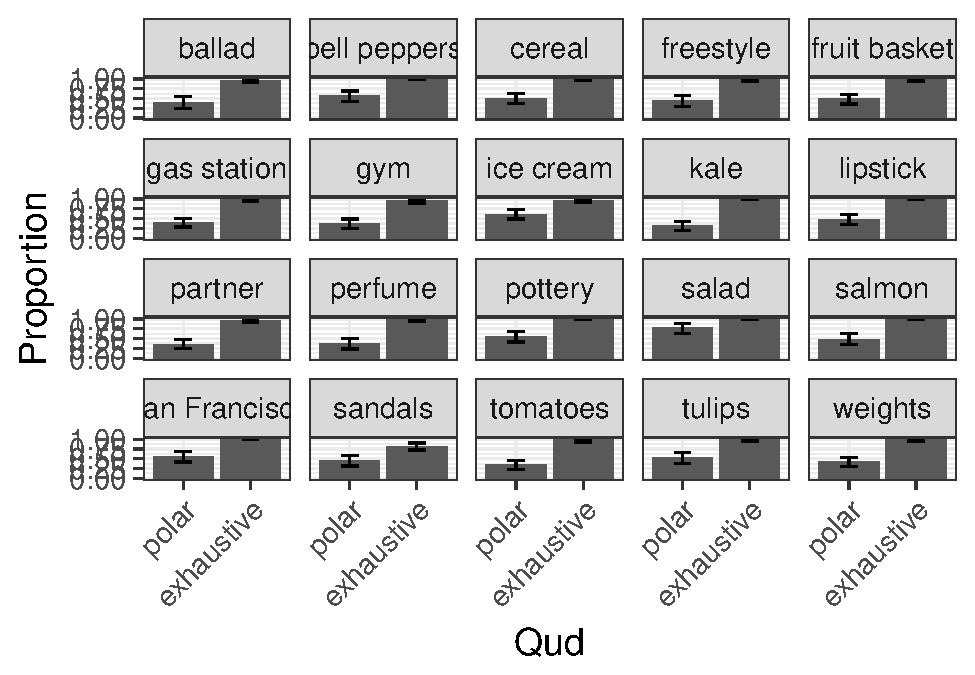
\includegraphics{visualizations_files/figure-latex/unnamed-chunk-23-1.pdf}

\begin{enumerate}
\def\labelenumi{\arabic{enumi}.}
\setcounter{enumi}{13}
\tightlist
\item
  Mean slider response over sensitivity score as a scatterplot (each dot
  is a subject)
\end{enumerate}

\begin{Shaded}
\begin{Highlighting}[]
\NormalTok{means =}\StringTok{ }\NormalTok{exhaustivity }\OperatorTok
\StringTok{  }\KeywordTok{group_by}\NormalTok{(qud,workerid) }\OperatorTok
\StringTok{  }\KeywordTok{summarise}\NormalTok{(}\DataTypeTok{Mean =} \KeywordTok{mean}\NormalTok{(response),}\DataTypeTok{CILow=}\KeywordTok{ci.low}\NormalTok{(response),}\DataTypeTok{CIHigh=}\KeywordTok{ci.high}\NormalTok{(response))}\OperatorTok
\StringTok{  }\KeywordTok{ungroup}\NormalTok{() }\OperatorTok
\StringTok{  }\KeywordTok{mutate}\NormalTok{(}\DataTypeTok{YMin=}\NormalTok{Mean}\OperatorTok{-}\NormalTok{CILow,}\DataTypeTok{YMax=}\NormalTok{Mean}\OperatorTok{+}\NormalTok{CIHigh) }\OperatorTok
\StringTok{  }\KeywordTok{mutate}\NormalTok{(}\DataTypeTok{Mean_New =}\NormalTok{ Mean,}\DataTypeTok{YMin_New =}\NormalTok{ YMin, }\DataTypeTok{YMax_New =}\NormalTok{ YMax) }\OperatorTok
\StringTok{  }\KeywordTok{mutate}\NormalTok{(}\DataTypeTok{Qud =} \KeywordTok{fct_reorder}\NormalTok{(qud,Mean)) }\OperatorTok
\StringTok{  }\KeywordTok{right_join}\NormalTok{(sensitivity,}\DataTypeTok{by=}\KeywordTok{c}\NormalTok{(}\StringTok{"workerid"}\NormalTok{))}

\KeywordTok{ggplot}\NormalTok{(means, }\KeywordTok{aes}\NormalTok{(}\DataTypeTok{x=}\NormalTok{sensitivityScore,}\DataTypeTok{y=}\NormalTok{Mean,}\DataTypeTok{color=}\NormalTok{Qud)) }\OperatorTok{+}
\StringTok{  }\KeywordTok{geom_point}\NormalTok{() }\OperatorTok{+}
\StringTok{  }\KeywordTok{geom_errorbar}\NormalTok{(}\KeywordTok{aes}\NormalTok{(}\DataTypeTok{ymin=}\NormalTok{YMin_New,}\DataTypeTok{ymax=}\NormalTok{YMax_New)) }\OperatorTok{+}\StringTok{ }
\StringTok{  }\KeywordTok{geom_smooth}\NormalTok{(}\DataTypeTok{method=}\StringTok{'lm'}\NormalTok{)}
\end{Highlighting}
\end{Shaded}

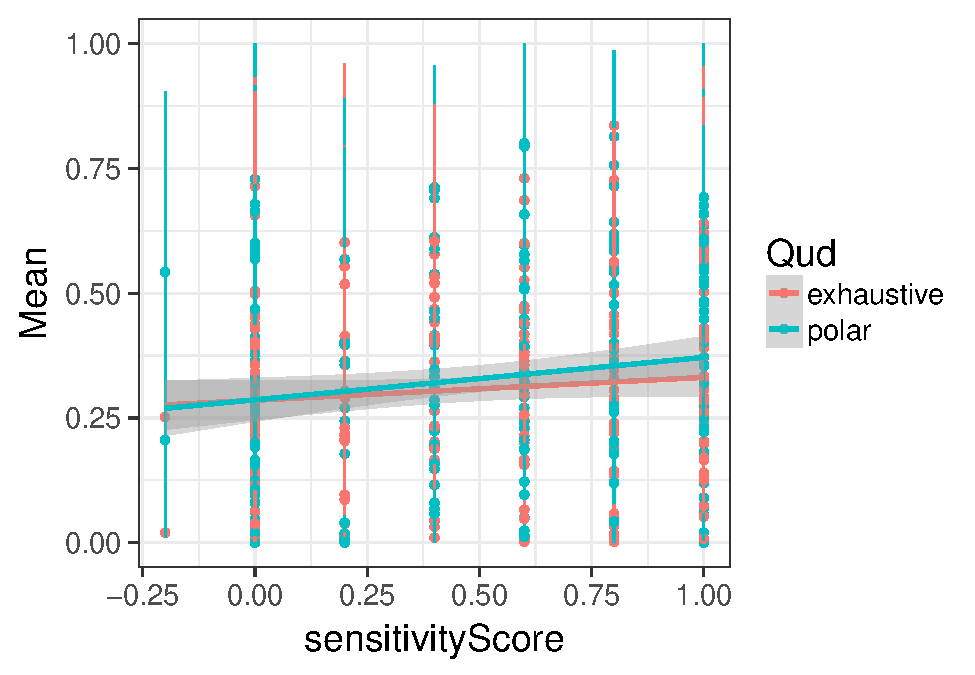
\includegraphics{visualizations_files/figure-latex/unnamed-chunk-24-1.pdf}

\begin{enumerate}
\def\labelenumi{\arabic{enumi}.}
\setcounter{enumi}{14}
\tightlist
\item
  Mean slider response over sensitivity score as a scatterplot (each dot
  is an item)
\end{enumerate}

\begin{Shaded}
\begin{Highlighting}[]
\NormalTok{means =}\StringTok{ }\NormalTok{exhaustivity }\OperatorTok
\StringTok{  }\KeywordTok{group_by}\NormalTok{(qud,topic) }\OperatorTok
\StringTok{  }\KeywordTok{summarise}\NormalTok{(}\DataTypeTok{Mean =} \KeywordTok{mean}\NormalTok{(response),}\DataTypeTok{CILow=}\KeywordTok{ci.low}\NormalTok{(response),}\DataTypeTok{CIHigh=}\KeywordTok{ci.high}\NormalTok{(response))}\OperatorTok
\StringTok{  }\KeywordTok{ungroup}\NormalTok{() }\OperatorTok
\StringTok{  }\KeywordTok{mutate}\NormalTok{(}\DataTypeTok{YMin=}\NormalTok{Mean}\OperatorTok{-}\NormalTok{CILow,}\DataTypeTok{YMax=}\NormalTok{Mean}\OperatorTok{+}\NormalTok{CIHigh) }\OperatorTok
\StringTok{  }\KeywordTok{mutate}\NormalTok{(}\DataTypeTok{Mean_New =}\NormalTok{ Mean,}\DataTypeTok{YMin_New =}\NormalTok{ YMin, }\DataTypeTok{YMax_New =}\NormalTok{ YMax) }\OperatorTok
\StringTok{  }\KeywordTok{mutate}\NormalTok{(}\DataTypeTok{Qud =} \KeywordTok{fct_reorder}\NormalTok{(qud,Mean)) }\OperatorTok
\StringTok{  }\KeywordTok{right_join}\NormalTok{(sensitivityItem,}\DataTypeTok{by=}\KeywordTok{c}\NormalTok{(}\StringTok{"topic"}\NormalTok{))}
\end{Highlighting}
\end{Shaded}

\begin{verbatim}
## Warning: Column `topic` joining character vector and factor, coercing into
## character vector
\end{verbatim}

\begin{Shaded}
\begin{Highlighting}[]
\KeywordTok{ggplot}\NormalTok{(means, }\KeywordTok{aes}\NormalTok{(}\DataTypeTok{x=}\NormalTok{sensitivityScoreItem,}\DataTypeTok{y=}\NormalTok{Mean,}\DataTypeTok{color=}\NormalTok{Qud)) }\OperatorTok{+}
\StringTok{  }\KeywordTok{geom_point}\NormalTok{() }\OperatorTok{+}
\StringTok{  }\KeywordTok{geom_errorbar}\NormalTok{(}\KeywordTok{aes}\NormalTok{(}\DataTypeTok{ymin=}\NormalTok{YMin_New,}\DataTypeTok{ymax=}\NormalTok{YMax_New)) }\OperatorTok{+}\StringTok{ }
\StringTok{  }\KeywordTok{geom_smooth}\NormalTok{(}\DataTypeTok{method=}\StringTok{'lm'}\NormalTok{)}
\end{Highlighting}
\end{Shaded}

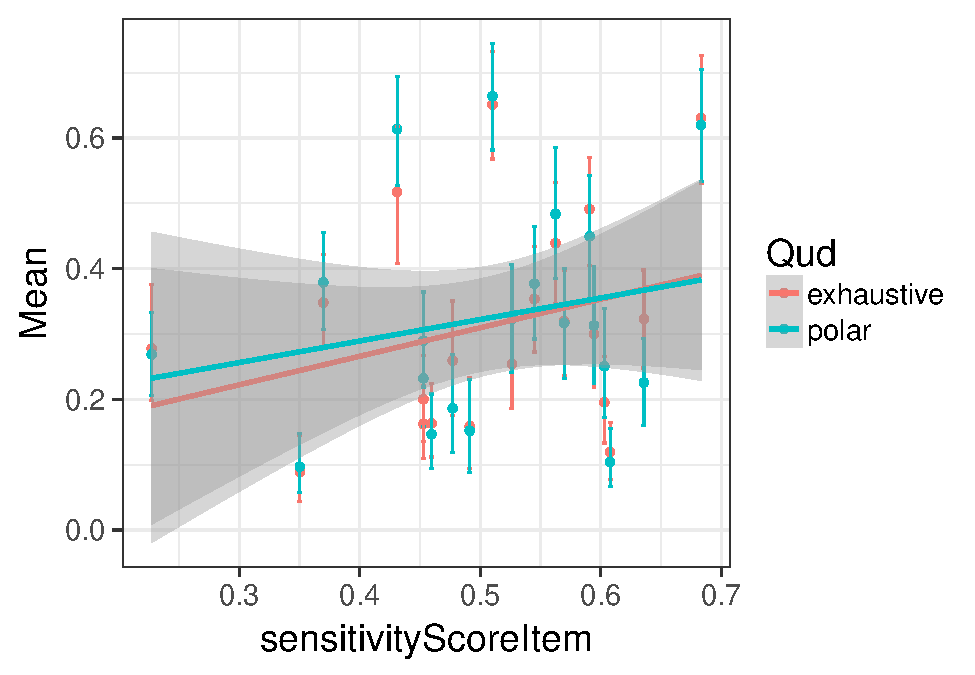
\includegraphics{visualizations_files/figure-latex/unnamed-chunk-25-1.pdf}

\begin{enumerate}
\def\labelenumi{\arabic{enumi}.}
\setcounter{enumi}{15}
\tightlist
\item
  Slider response over sensitivity score per trial as a scatterplot
\end{enumerate}

\begin{Shaded}
\begin{Highlighting}[]
\KeywordTok{ggplot}\NormalTok{(exhaustivity, }\KeywordTok{aes}\NormalTok{(}\DataTypeTok{x=}\NormalTok{sensitivityScore,}\DataTypeTok{y=}\NormalTok{response,}\DataTypeTok{color=}\NormalTok{qud)) }\OperatorTok{+}
\StringTok{  }\KeywordTok{geom_point}\NormalTok{() }\OperatorTok{+}
\StringTok{  }\KeywordTok{geom_smooth}\NormalTok{(}\DataTypeTok{method=}\StringTok{'lm'}\NormalTok{)}
\end{Highlighting}
\end{Shaded}

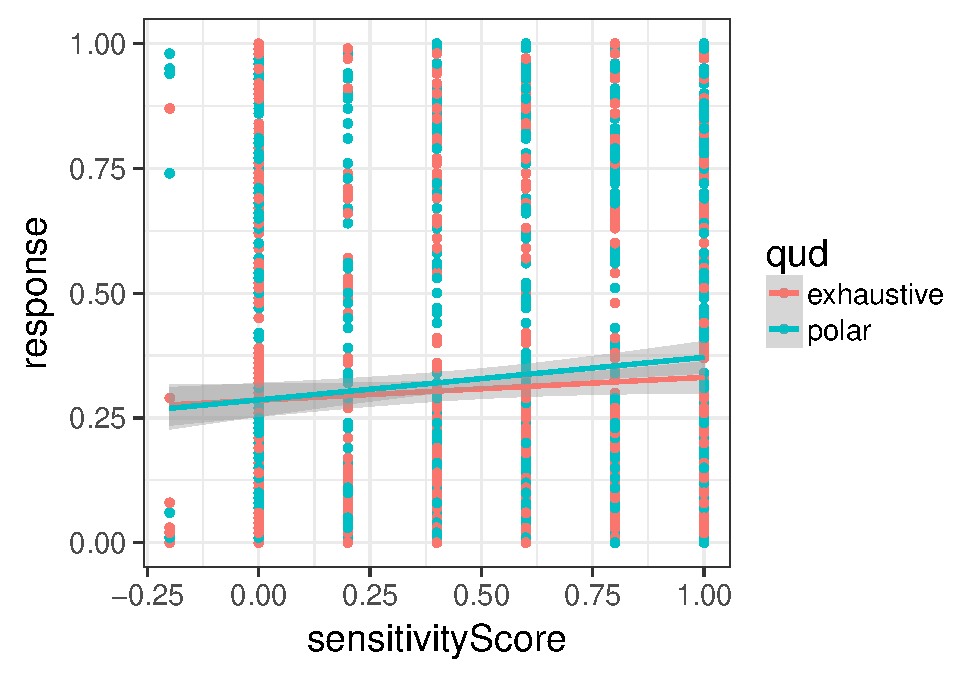
\includegraphics{visualizations_files/figure-latex/unnamed-chunk-26-1.pdf}

\begin{enumerate}
\def\labelenumi{\arabic{enumi}.}
\setcounter{enumi}{16}
\tightlist
\item
  Mean slider response over prior beliefs as a scatterplot (each dot is
  an item)
\end{enumerate}

\begin{Shaded}
\begin{Highlighting}[]
\NormalTok{means =}\StringTok{ }\NormalTok{exhaustivity }\OperatorTok
\StringTok{  }\KeywordTok{group_by}\NormalTok{(qud,topic) }\OperatorTok
\StringTok{  }\KeywordTok{summarise}\NormalTok{(}\DataTypeTok{Mean =} \KeywordTok{mean}\NormalTok{(response),}\DataTypeTok{CILow=}\KeywordTok{ci.low}\NormalTok{(response),}\DataTypeTok{CIHigh=}\KeywordTok{ci.high}\NormalTok{(response))}\OperatorTok
\StringTok{  }\KeywordTok{ungroup}\NormalTok{() }\OperatorTok
\StringTok{  }\KeywordTok{mutate}\NormalTok{(}\DataTypeTok{YMin=}\NormalTok{Mean}\OperatorTok{-}\NormalTok{CILow,}\DataTypeTok{YMax=}\NormalTok{Mean}\OperatorTok{+}\NormalTok{CIHigh) }\OperatorTok
\StringTok{  }\KeywordTok{mutate}\NormalTok{(}\DataTypeTok{Mean_New =}\NormalTok{ Mean,}\DataTypeTok{YMin_New =}\NormalTok{ YMin, }\DataTypeTok{YMax_New =}\NormalTok{ YMax) }\OperatorTok
\StringTok{  }\KeywordTok{mutate}\NormalTok{(}\DataTypeTok{Qud =} \KeywordTok{fct_reorder}\NormalTok{(qud,Mean)) }\OperatorTok
\StringTok{  }\KeywordTok{left_join}\NormalTok{(priorsItems,}\DataTypeTok{by=}\KeywordTok{c}\NormalTok{(}\StringTok{"topic"}\NormalTok{))}
\end{Highlighting}
\end{Shaded}

\begin{verbatim}
## Warning: Column `topic` joining character vector and factor, coercing into
## character vector
\end{verbatim}

\begin{Shaded}
\begin{Highlighting}[]
\KeywordTok{ggplot}\NormalTok{(means, }\KeywordTok{aes}\NormalTok{(}\DataTypeTok{x=}\NormalTok{Mean_Prior,}\DataTypeTok{y=}\NormalTok{Mean_New,}\DataTypeTok{color=}\NormalTok{Qud)) }\OperatorTok{+}
\StringTok{  }\KeywordTok{geom_point}\NormalTok{() }\OperatorTok{+}
\StringTok{  }\KeywordTok{geom_errorbar}\NormalTok{(}\KeywordTok{aes}\NormalTok{(}\DataTypeTok{ymin=}\NormalTok{YMin_New,}\DataTypeTok{ymax=}\NormalTok{YMax_New)) }\OperatorTok{+}\StringTok{ }
\StringTok{  }\KeywordTok{geom_errorbarh}\NormalTok{(}\KeywordTok{aes}\NormalTok{(}\DataTypeTok{xmin=}\NormalTok{YMin_Prior,}\DataTypeTok{xmax=}\NormalTok{YMax_Prior)) }\OperatorTok{+}\StringTok{ }
\StringTok{  }\KeywordTok{geom_smooth}\NormalTok{(}\DataTypeTok{method=}\StringTok{'lm'}\NormalTok{)}
\end{Highlighting}
\end{Shaded}

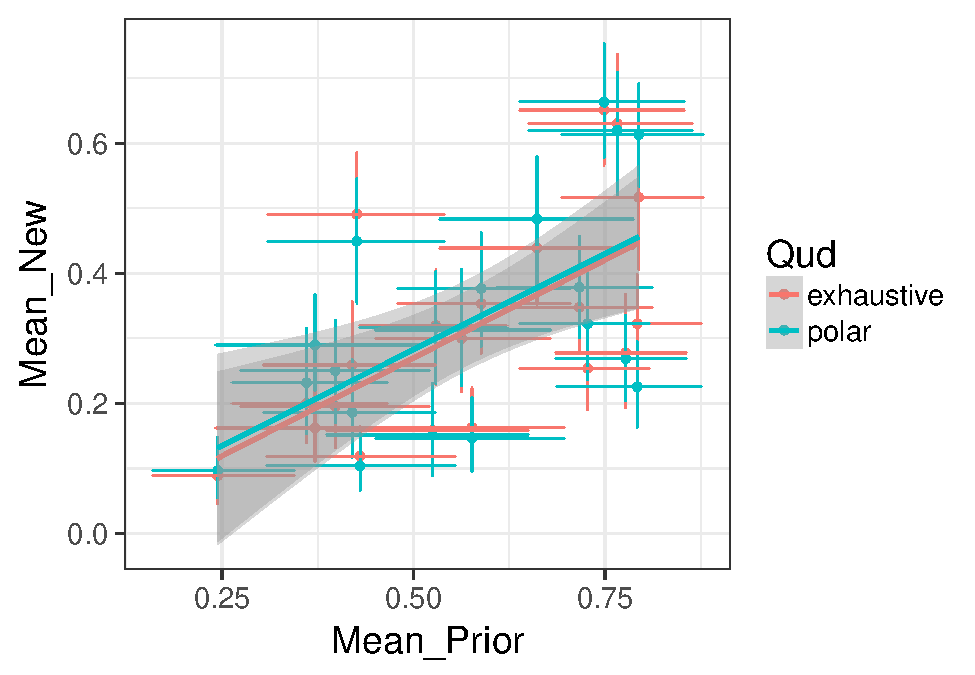
\includegraphics{visualizations_files/figure-latex/unnamed-chunk-27-1.pdf}

\subsection{Part 8: Analysis}\label{part-8-analysis}

\begin{Shaded}
\begin{Highlighting}[]
\NormalTok{ad =}\StringTok{ }\NormalTok{exhaustivity }\OperatorTok
\StringTok{     }\KeywordTok{droplevels}\NormalTok{() }\OperatorTok
\StringTok{     }\KeywordTok{mutate}\NormalTok{(}\DataTypeTok{Topic =} \KeywordTok{as.factor}\NormalTok{(}\KeywordTok{as.character}\NormalTok{(topic))) }\OperatorTok
\StringTok{     }\KeywordTok{mutate}\NormalTok{(}\DataTypeTok{Prior =} \KeywordTok{as.numeric}\NormalTok{(}\KeywordTok{as.character}\NormalTok{(Mean_Prior))) }\OperatorTok
\StringTok{     }\KeywordTok{mutate}\NormalTok{(}\DataTypeTok{cqud =} \KeywordTok{myCenter}\NormalTok{(qud), }\DataTypeTok{cSensitivity =} \KeywordTok{myCenter}\NormalTok{(sensitivityScore),}\DataTypeTok{cPrior =} \KeywordTok{myCenter}\NormalTok{(Prior))}

\KeywordTok{nrow}\NormalTok{(ad)}
\end{Highlighting}
\end{Shaded}

\begin{verbatim}
## [1] 2250
\end{verbatim}

\begin{Shaded}
\begin{Highlighting}[]
\KeywordTok{library}\NormalTok{(lme4)}

\NormalTok{m =}\StringTok{ }\KeywordTok{lmer}\NormalTok{(response }\OperatorTok{~}\StringTok{ }\NormalTok{cqud }\OperatorTok{*}\StringTok{ }\NormalTok{cPrior }\OperatorTok{*}\StringTok{ }\NormalTok{cSensitivity }\OperatorTok{+}\StringTok{ }\NormalTok{(}\DecValTok{1} \OperatorTok{+}\StringTok{ }\NormalTok{cqud}\OperatorTok{*}\NormalTok{cPrior}\OperatorTok{*}\NormalTok{cSensitivity }\OperatorTok{|}\NormalTok{Topic) }\OperatorTok{+}\StringTok{ }\NormalTok{(}\DecValTok{1} \OperatorTok{+}\StringTok{ }\NormalTok{cqud}\OperatorTok{*}\NormalTok{cPrior}\OperatorTok{*}\NormalTok{cSensitivity}\OperatorTok{|}\NormalTok{workerid), }\DataTypeTok{data=}\NormalTok{ad)}
\end{Highlighting}
\end{Shaded}

\begin{verbatim}
## Warning in commonArgs(par, fn, control, environment()): maxfun < 10 *
## length(par)^2 is not recommended.
\end{verbatim}

\begin{verbatim}
## Warning in optwrap(optimizer, devfun, getStart(start, rho$lower, rho$pp), :
## convergence code 1 from bobyqa: bobyqa -- maximum number of function
## evaluations exceeded
\end{verbatim}

\begin{verbatim}
## Warning in checkConv(attr(opt, "derivs"), opt$par, ctrl = control
## $checkConv, : unable to evaluate scaled gradient
\end{verbatim}

\begin{verbatim}
## Warning in checkConv(attr(opt, "derivs"), opt$par, ctrl = control
## $checkConv, : Model failed to converge: degenerate Hessian with 1 negative
## eigenvalues
\end{verbatim}

\begin{Shaded}
\begin{Highlighting}[]
\KeywordTok{summary}\NormalTok{(m)}
\end{Highlighting}
\end{Shaded}

\begin{verbatim}
## Linear mixed model fit by REML ['lmerMod']
## Formula: response ~ cqud * cPrior * cSensitivity + (1 + cqud * cPrior *  
##     cSensitivity | Topic) + (1 + cqud * cPrior * cSensitivity |  
##     workerid)
##    Data: ad
## 
## REML criterion at convergence: 794.1
## 
## Scaled residuals: 
##     Min      1Q  Median      3Q     Max 
## -3.0611 -0.6211 -0.1699  0.4987  3.5640 
## 
## Random effects:
##  Groups   Name                     Variance  Std.Dev. Corr             
##  workerid (Intercept)              1.549e-02 0.124446                  
##           cqud                     1.019e-02 0.100961  0.15            
##           cPrior                   5.071e-02 0.225192  0.98 -0.07      
##           cSensitivity             1.321e-03 0.036340 -0.29  0.55 -0.41
##           cqud:cPrior              9.189e-02 0.303137  0.18  1.00 -0.04
##           cqud:cSensitivity        7.468e-03 0.086418  0.04  0.99 -0.17
##           cPrior:cSensitivity      2.975e-02 0.172479 -0.04 -0.94  0.16
##           cqud:cPrior:cSensitivity 1.845e-01 0.429555 -0.55 -0.88 -0.37
##  Topic    (Intercept)              1.454e-02 0.120589                  
##           cqud                     3.864e-05 0.006216 -0.34            
##           cPrior                   4.039e-02 0.200966  0.99 -0.22      
##           cSensitivity             2.413e-03 0.049117  0.68  0.44  0.75
##           cqud:cPrior              2.283e-02 0.151081  0.54 -0.61  0.41
##           cqud:cSensitivity        1.256e-03 0.035439  0.52  0.20  0.64
##           cPrior:cSensitivity      8.856e-03 0.094108  0.49 -0.28  0.39
##           cqud:cPrior:cSensitivity 4.489e-01 0.669970  1.00 -0.41  0.98
##  Residual                          6.754e-02 0.259879                  
##                         
##                         
##                         
##                         
##                         
##   0.48                  
##   0.55  0.99            
##  -0.31 -0.96 -0.96      
##  -0.45 -0.88 -0.83  0.74
##                         
##                         
##                         
##                         
##   0.15                  
##   0.54 -0.43            
##   0.36  0.93 -0.44      
##   0.62  0.55  0.51  0.47
##                         
## Number of obs: 2250, groups:  workerid, 225; Topic, 20
## 
## Fixed effects:
##                          Estimate Std. Error t value
## (Intercept)              0.314801   0.029309  10.741
## cqud                     0.009853   0.014137   0.697
## cPrior                   0.509612   0.121241   4.203
## cSensitivity             0.072459   0.028470   2.545
## cqud:cPrior              0.013185   0.083394   0.158
## cqud:cSensitivity        0.005722   0.038774   0.148
## cPrior:cSensitivity      0.148118   0.115620   1.281
## cqud:cPrior:cSensitivity 0.112183   0.248339   0.452
## 
## Correlation of Fixed Effects:
##             (Intr) cqud   cPrior cSnstv cqd:cP cqd:cS cPrr:S
## cqud         0.010                                          
## cPrior       0.534  0.119                                   
## cSensitivty  0.236  0.081  0.155                            
## cqud:cPrior  0.198  0.057 -0.012 -0.027                     
## cqd:cSnstvt  0.190  0.215  0.426  0.122 -0.072              
## cPrr:cSnstv  0.143 -0.061  0.265  0.291  0.068  0.059       
## cqd:cPrr:cS  0.528 -0.081  0.143  0.146  0.108  0.106  0.042
## convergence code: 1
## unable to evaluate scaled gradient
## Model failed to converge: degenerate  Hessian with 1 negative eigenvalues
## maxfun < 10 * length(par)^2 is not recommended.
\end{verbatim}


\end{document}
